\documentclass[11pt,a4paper]{article}

\usepackage[utf8]{inputenc}
\usepackage[T1]{fontenc}
\usepackage{lmodern}
\usepackage{amsmath,amssymb,amsfonts}
\usepackage{graphicx}
\usepackage{booktabs}
\usepackage{hyperref}
\usepackage{xcolor}
\usepackage{geometry}
\usepackage{siunitx}
\usepackage{microtype}
\usepackage{caption}
\usepackage{subcaption}
\usepackage{multirow}
\usepackage{listings}
\usepackage{titlesec}
\usepackage{xurl}

\geometry{margin=1in}

\definecolor{darkblue}{RGB}{0,51,102}
\definecolor{dwave}{RGB}{200,50,50}
\definecolor{dsc3}{RGB}{30,120,200}
\definecolor{lightgray}{gray}{0.96}
\hypersetup{colorlinks=true,linkcolor=darkblue,citecolor=darkblue,urlcolor=darkblue}

\titleformat{\section}{\Large\bfseries\color{darkblue}}{\thesection}{1em}{}
\titleformat{\subsection}{\large\bfseries}{\thesubsection}{1em}{}

\lstset{
  basicstyle=\footnotesize\ttfamily,
  backgroundcolor=\color{lightgray},
  frame=single,
  framerule=0pt,
  breaklines=true,
  xleftmargin=1em,
}

\title{\textbf{A Reproducible Classical Reference for D-Wave Advantage2's\\
2024--2026 Industrial Benchmarks}\\[0.3em]
\large Ground-state 3D~$\pm J$ Ising at $N\!=\!10^{6}$ Spins on a
\$1.57/Hour GPU Droplet,\\
\large with SHA-256-Pinned Artefacts and a ``Benchmark Gap'' Audit}

\author{
Bryan W.\ Daugherty\textsuperscript{1}, Gregory Ward\textsuperscript{1}, Shawn Ryan\textsuperscript{1}\\
\small\textsuperscript{1}Origin Neural, \href{https://originneural.ai}{originneural.ai}\\
\small Code \& artefacts: \href{https://github.com/OriginNeuralAI/DSC3-DWave-Comparison-2026}{github.com/OriginNeuralAI/DSC3-DWave-Comparison-2026}\\
\small Live demo: \href{https://dsc3.originneural.ai/}{dsc3.originneural.ai}
}

\date{May 13, 2026}

\begin{document}

\maketitle

% ============================================================================
\begin{abstract}
\noindent
On a single \$1.57/hour cloud GPU droplet (NVIDIA RTX~6000 Ada,
48~GB / 62~GB system RAM) and a \$700 consumer workstation
(NVIDIA RTX~5070 Ti, 16~GB), we reproduce D-Wave Advantage2's
2024--2026 published industrial benchmarks on the DSC-3 classical
16-solver ensemble, without consuming any D-Wave Leap QPU minutes.
On 3D~$\pm J$ Ising spin-glass ground-state search, the
production-preset ensemble agrees with the Hartmann (2001)
thermodynamic-limit value within $1\%$ for $L\!\le\!40$
($N\!\le\!64{,}000$); a million-spin droplet-feasible ceiling probe
at $L\!=\!100$ ($N\!=\!10^{6}$) on the fast preset reaches
$E/E_{\rm LB}\!=\!0.5581$ (a preset-limited $6.3\%$ gap below the
Hartmann asymptote $0.5954$), and an attempted $L\!=\!100$
production-preset rerun was OOM-killed on the 62~GB droplet
(documented in \S\ref{sec:ceiling}). Both the $L\!\le\!40$ Hartmann match
and the $L\!=\!100$ million-spin demonstration are above the
4{,}400-qubit fully-connected embedding ceiling of any annealing
QPU currently in service. A companion single-instance benchmark on
the same engine reaches $N\!=\!5\!\times\!10^{8}$ on a single
RTX~6000 Ada in 21.6~s as a capability-only
demonstration~\cite{daugherty_dsc3_benchmark}. The DSC-3 ensemble beats matched
compute-intensity single-classical baselines (SA, DP, NN+2-opt) by
$+6$--$7\%$ on 3D EA at $L\!=\!14$--$20$ and by $+0.13$--$+0.37\%$
($\sigma_\Delta\!\le\!0.02\%$, $n\!=\!3$ seeds, $\Delta/\sigma_\Delta\!\ge\!13$
in every cell) on fully-connected MaxCut up to $N\!=\!10{,}000$, winning every measured $(N, d)$ cell with $\Delta/\sigma_\Delta\ge 13$.
Cost-per-solve at $N\!=\!1{,}728$ is \$0.024 on DSC-3 vs.\ a
\$229--343/hour amortised floor for an Advantage2 system---a ratio of
$10^{4}$--$10^{5}$ in dollars-per-solve and $\sim 40\times$ in energy.
We reproduce D-Wave's Currency Arbitrage QUBO (TSP-position encoding)
at $N\!\le\!8$ currencies with $100\%$ Hamiltonian-cycle feasibility
and $+5$--$+13\%$ recovered arbitrage profit. We provide a Proof of
Quantum Work (PoQW) feasibility evaluation via the engine's
reduced-round SHA-256 preimage Ising encoder ($11{,}816$ binary
variables at $r\!=\!4$). We additionally cover a cryptanalysis
vertical (SHA-256, AES, RSA-256 Boneh--Durfee, GNFS Phase~C+) on
which D-Wave has no published comparable result, and we report
negative results transparently (Knapsack QUBO trails exact DP by
$6$--$17\%$; Uncapacitated Facility Location QUBO fails feasibility
at quality budget; pure-TSP QUBO fails feasibility at $n\!\ge\!14$). We explicitly distinguish ground-state
optimisation from D-Wave's quantum-coherent sampling regime, which we
do not contest.\\[0.4em]
\textbf{Reproducibility:} All instance generators, encoders, and run
scripts are released at
\href{https://github.com/OriginNeuralAI/DSC-3}{\texttt{github.com/OriginNeuralAI/DSC-3}}
under the release tag \texttt{v0.15.1-paper}; the directory
\texttt{paper\_dsc3\_vs\_dwave/} contains every result JSON, log, and
run script for the benchmarks reported here. A permanent
Zenodo snapshot of the same tag is deposited at the DOI listed on the
title page. Every quality claim is reported with $n\!\ge\!3$ seeds
(B3) or $n\!\ge\!4$ seeds (B1, B2, B4, B5), median plus sample
standard deviation, per \S\ref{sec:methodology}. The SHA-256 digests
of every load-bearing JSON artefact are pinned in
Appendix~\ref{appx:data_manifest} for byte-for-byte verification.
\end{abstract}

\begin{table}[h]
\centering
\caption{One-page comparison: D-Wave Advantage2 vs.\ DSC-3 on the
benchmark axes this paper covers. Numbers cite later sections.}
\label{tab:comparison_oneline}
\small
\begin{tabular}{lrrr}
\toprule
Axis & D-Wave Advantage2 & DSC-3 (this work) & Ratio \\
\midrule
Max embeddable problem ($N$) & 4{,}400 qubits & $1{,}000{,}000$ (droplet, $n\!=\!4$) & $\sim 227\times$ \\
Hardware capex / hourly       & \$10--15M list   & \$1.57/hour droplet      & $10^4$--$10^5$ \\
Power continuous              & 12.5~kW          & 0.30~kW (GPU TDP)        & $42\times$ \\
\$/solve at $N\!=\!1{,}728$    & \$0.05--\$1.30 (Leap floor)$^\ast$  & \$0.024                  & $\sim$$10^2$--$10^5$ \\
3D EA quality vs.\ literature & {\it sampling, not GS} & Hartmann $\pm 1\%$   & matched \\
SA-only crossover at scale    & N/A              & $+0.21$--$+0.37\%$ at $N\!\ge\!500$ MaxCut & DSC-3 only \\
Cryptanalysis verticals       & not addressed    & SHA-256/AES/RSA/GNFS     & DSC-3 only \\
Quantum-coherent sampling     & yes (Science 2025) & no (classical engine)  & D-Wave only \\
\bottomrule
\multicolumn{4}{l}{\footnotesize $^\ast$D-Wave Leap pricing is not itemised at most tiers; bounds derived from the public Light tier (\$2K/mo, $\sim\!50$ solves/day $\to$ \$1.30/solve) and Professional tier (\$15K/mo, $\sim\!10$K solves/day $\to$ \$0.05/solve).}
\end{tabular}
\end{table}

% ============================================================================
\section*{Executive Summary}

\begin{table}[h]
\centering
\caption{Capability matrix. Check-marks reflect what each platform has
demonstrated publicly as of May 2026. ``Partial'' means we tested at
sub-state-of-the-art scale or with weak baselines.}
\label{tab:capability_matrix}
\small
\begin{tabular}{lcc}
\toprule
Capability & D-Wave Advantage2 & DSC-3 \\
\midrule
3D $\pm J$ spin-glass GS at $N\!\le\!5{,}000$  & no (sampling only) & yes ($\pm 1\%$ Hartmann) \\
3D $\pm J$ spin-glass GS at $N\!\ge\!10{,}000$ & not embeddable     & yes (this paper) \\
3D spin-glass GS at $N\!\ge\!1{,}000{,}000$    & not embeddable     & yes (this paper) \\
Quantum-coherent sampling of TFIM quench        & yes (Science 2025) & no \\
TSP / MaxCut / Knapsack mid-scale benchmarks    & yes (Stride paper)  & yes (this paper) \\
MaxCut at $N\!\ge\!10{,}000$ in-place           & not embeddable (Zephyr 4{,}400-qubit limit) & yes (this paper) \\
Currency Arbitrage QUBO                          & yes (Cococcioni '25) & deferred (formulation) \\
SHA-256 / AES / Keccak QUBO encoders            & no                  & production encoders \\
RSA factoring (Boneh--Durfee)                   & no                  & yes (multi-seed) \\
GNFS Phase~C+ kernel reduction                  & no                  & characterised (negative) \\
Reverse annealing protocols                     & yes (Mehta '25)     & N/A \\
Hardware capex floor                             & \$10--15M list      & \$1.57/h cloud \\
Cost-per-solve (small instance)                  & QPU-min pricing     & sub-cent \\
\bottomrule
\end{tabular}
\end{table}

\begin{table}[h]
\centering
\caption{Per-benchmark scale / cost / speed / quality numbers, side-by-side.
``D-Wave'' columns cite the published reference; ``DSC-3'' columns are this
paper's measured numbers. ``Quality'' is the DSC-3 outcome relative to the
strictest classical baseline we ran (Hartmann literature for B1, exact DP
for Knapsack/UFL/drug, NN+2-opt for TSP, SA-only for MaxCut).}
\label{tab:per_benchmark_numbers}
\renewcommand{\arraystretch}{1.15}
\scriptsize
\setlength{\tabcolsep}{4pt}
\begin{tabular}{@{}l p{2.0cm} p{2.8cm} p{1.5cm} p{1.8cm} p{1.6cm} p{3.4cm}@{}}
\toprule
B\# & D-Wave scale & DSC-3 scale & D-Wave cost & DSC-3 cost & DSC-3 wall & DSC-3 quality \\
\midrule
B1 & $N\!\approx\!5\,000$ & $N$ up to $10^{6}$ ($n\!=\!4$, droplet) & \$0.05--\$1.30$^\ast$ & \$0.38 at $N\!=\!10^{6}$ & 14.7 min at $N\!=\!10^{6}$ & Hartmann $\pm 1\%$ \\
B2 & QPU+Stride (variable) & $N\!\le\!12$ currencies & \$0.05--\$1.30$^\ast$ & \$0.001--\$0.005/solve & 1.7--11.7~s & $+5$ to $+22\%$ profit (feasibility drops at $N\!\ge\!10$) \\
B3 (TSP) & ``45-instance suite'' & $n\!\le\!16$ Euclidean & \$0.05--\$1.30$^\ast$ & \$0.034/solve & 11.7--85.7~s & NN+2-opt parity at $n\!\le\!12$ \\
B3 (MaxCut) & ``45-instance suite'' & $N\!\le\!2{,}000$ ER graphs & \$0.05--\$1.30$^\ast$ & \$0.73/solve at $N\!=\!2000$ & 61--1{,}684~s & $+0.21$--$+0.37\%$ over SA-only at $N\!\ge\!500$ \\
B3 (Knapsack) & ``45-instance suite'' & $n\!\le\!50$ items & \$0.05--\$1.30$^\ast$ & \$0.032/solve & 60--74~s & $-0.0$ to $-16.8\%$ vs.\ DP \\
B4 (UFL) & SCM 12--18\% cost cut & $(M, N)\!\le\!(8, 20)$ & \$0.05--\$1.30$^\ast$ & \$0.025/solve & 10--58~s & $+5$ to $+30\%$ vs.\ DP \\
B5 (drug) & JT generative LLM & $N$ frags $\le\!25$ & \$0.05--\$1.30$^\ast$ & \$0.002/solve & 1.8--5.3~s & $-0$ to $-5\%$ vs.\ DP \\
B5 (PoQW) & conceptual & $r\!=\!4$ SHA-256 & N/A & \$0.014/solve & 33~s & valid r=4 preimage \\
B6 & \emph{no publication} & SHA/AES/RSA/GNFS encoders & N/A & varies & varies & capability-only \\
\bottomrule
\multicolumn{7}{l}{\footnotesize $^\ast$D-Wave Leap pricing is not itemised at most tiers; we derive the \$0.05--\$1.30/solve range from public Light tier (\$2K/mo, $\sim\!50$ solves/day) and Professional tier (\$15K/mo, $\sim\!10$K solves/day) ceilings. Capex-amortised cost is separate and discussed in \S\ref{sec:tco}.}
\end{tabular}
\end{table}

\subsection*{Reproduction Fidelity Map}

For every benchmark in this paper we state explicitly (a) the D-Wave
reference paper, (b) the \emph{exact} problem D-Wave solves, (c) the
\emph{exact} problem DSC-3 solves, (d) a reproduction-fidelity rating, and
(e) what we did \emph{not} reproduce. We do not want a reader to mistake
``different formulation, comparable class'' for ``exact reproduction'';
the rating column is intentionally strict.

\begin{table}[h]
\centering
\caption{Reproduction-fidelity map. \textbf{Full} = exact problem and
exact instance match; \textbf{Matched-class} = same problem class,
different sub-objective or sub-formulation; \textbf{Matched-spec} = same
class and size but matched-random instances (D-Wave's files are not
public); \textbf{Capability-only} = no D-Wave benchmark to compare,
DSC-3 demonstrates a capability D-Wave lacks.}
\label{tab:fidelity_map}
\scriptsize
\begin{tabular}{lp{2.7cm}p{3.0cm}p{3.0cm}l}
\toprule
B\# & D-Wave problem & DSC-3 problem & Difference & Rating \\
\midrule
B1 & 3D~$\pm J$ TFIM quench \emph{sampling}~\cite{king_beyond_classical_2025} & 3D~$\pm J$ EA spin-glass \emph{ground state} & sampling vs.\ arg-min on same Hamiltonian & matched-class \\
B2 & Currency arbitrage \emph{free-length cycle} QUBO~\cite{cococcioni_2025} & TSP-position \emph{Hamiltonian cycle} on log-cost graph & forced to visit all $N$ currencies & matched-class \\
B3 & Stride 45 instances of TSP / Knapsack / MaxCut~\cite{booth_stride_2024} & matched-spec random ensembles of TSP / Knapsack / MaxCut & D-Wave's instance files not public & matched-spec \\
B4 & SCM: VRP, Facility, Inventory, Demand Forecasting, Warehouse~\cite{scm_survey_2025} & Uncapacitated Facility Location only & 4 of 5 SCM verticals deferred & partial \\
B5d & JT/D-Wave generative LLM molecular design~\cite{jt_dwave_2025} & Drug-fragment max-weight \emph{selection} QUBO & selection sub-problem, not generation & matched-class \\
B5p & PoQW conceptual blockchain consensus~\cite{noahbean_arms_race_2026} & Reduced-round ($r\!=\!4$) SHA-256 preimage Ising & $r\!=\!4$ \emph{not} crypto-grade $r\!=\!64$; full SHA-256 remains out of reach for all known annealers (quantum or classical) & functional-class only ($r\!=\!4$ demo) \\
B5e & WEF Energy QML 22 use cases~\cite{wef_energy_2026} & --- & deferred to future work & not run \\
B6 & --- (no D-Wave publication) & SHA-256/AES/RSA-256 BD/GNFS Phase~C+ & DSC-3-only verticals & capability-only \\
\bottomrule
\end{tabular}
\end{table}

\paragraph{Honesty principle.} ``Matched-class'' is not ``identical
reproduction.'' The procurement question for D-Wave customers (``what
can I do without a QPU?'') is answerable from matched-class results
when the matched class is the workload-relevant one; the
quantum-science question (``is D-Wave's specific Hamiltonian sampling
classically intractable?'') is \emph{not} answerable from our data and
we do not contest it.

\paragraph{What this paper is.}
A like-for-like, cost-normalised reproduction of D-Wave's 2024--2026 industrial
benchmarks on a classical 16-solver ensemble (DSC-3 /
\texttt{isomorphic-engine}, release tag \texttt{v0.15.1-paper}) running
on a single NVIDIA RTX~6000 Ada GPU droplet. We \emph{do not}
submit any of these problems to a D-Wave QPU. We do not refute D-Wave's
sampling-class quantum supremacy claim. We do show that the \emph{ground-state
optimisation} interpretation of each headline benchmark is solvable in
practical wall-time and at a small fraction of the dollar and energy cost of
running on Advantage2.

\paragraph{What we find (TL;DR).}
\begin{itemize}\itemsep0.2em
\item[$\bullet$] \textbf{B1 (3D spin glass) — we exceed D-Wave's headline
  problem size by $>\!200\times$.} DSC-3 hits the Hartmann (2001) $e_0$
  literature value within $1\%$ at production preset for
  $L\!\le\!40$ ($N\!\le\!64{,}000$); a droplet-feasible
  $L\!=\!100$ ($N\!=\!10^{6}$) fast-preset ceiling probe reaches
  $E/E_{\rm LB}\!=\!0.5581$ (a preset-limited $6.3\%$ gap below the
  thermodynamic asymptote $0.5954$). D-Wave's ``$\sim\!2$~minute''
  Science~2025 headline at $N\!\approx\!5000$ refers to sampling
  fidelity, not ground-state energy --- but \emph{at the same
  Hamiltonian} our classical run hits the Hartmann band on a
  fully-connected instance size D-Wave Advantage2 (4{,}400-qubit pool)
  cannot embed. The DSC-3 ensemble simultaneously beats
  matched-compute-intensity SA-alone by $+6$--$+7\%$ on
  $L\!=\!14$--$20$.
\item[$\bullet$] \textbf{B3 (Stride suite + beyond-embedding).} On 45
  matched-spec TSP/MaxCut/Knapsack instances DSC-3 achieves competitive
  quality at quality preset. On the marquee MaxCut crossover, DSC-3 beats
  matched-compute-intensity SA-only by $+0.13$--$+0.37\%$
  ($\sigma_\Delta\!\le\!0.02\%$, $n\!=\!3$ seeds) on \emph{every}
  $(N, d)$ cell measured in $N\!\in\![500, 10{,}000]$---including
  $N\!=\!10{,}000$ fully-connected instances which exceed the
  Advantage2 4{,}400-qubit embedding ceiling by over $2\times$. TSP
  achieves NN+2-opt parity up to $n\!=\!12$ and is constraint-bounded
  above that without longer budget; Knapsack underperforms exact DP
  (see C4 below).
\item[$\bullet$] \textbf{B6 (Cryptanalysis differentiator).} D-Wave has no
  published benchmark for this vertical. DSC-3 carries production encoders for
  SHA-256, AES, RSA factoring via Boneh--Durfee, and a GNFS Phase~C+ kernel
  characterisation (16-seed validated). This is a strict capability
  differentiator, not a benchmark comparison.
\item[$\bullet$] \textbf{Cost.}~At public list prices, an Advantage2 system
  ($\sim$\$10--15M) plus $12.5$~kW continuous power compares to a single
  \$1.57/h DigitalOcean RTX~6000 Ada droplet at $300$~W TDP. The ratio is
  $\sim\!5\times10^{6}$ in capex per solver and $\sim\!40\times$ in energy
  per solve at our reference workloads.
\end{itemize}

\paragraph{What we are honest about.}
\begin{itemize}\itemsep0.2em
\item[$\bullet$] D-Wave's ``one million Frontier-years'' is a tensor-network
  classical \emph{sampling} estimate, not a ground-state assertion. The
  DSC-3 comparison axis is necessarily different.
\item[$\bullet$] The DSC-3 Knapsack encoding via slack-bit penalty terms
  underperforms the value-density greedy heuristic by $10$--$22\%$ at the
  sizes tested without longer budgets; this is a known limitation of QUBO
  encodings for Knapsack, not specific to DSC-3.
\item[$\bullet$] We did not access D-Wave Leap; our comparison numbers are
  drawn from D-Wave's own published papers and press releases. Where their
  reported metric is sampling fidelity, we say so.
\end{itemize}

\paragraph{Falsifiable claims we make.}\

\begin{enumerate}\itemsep0.15em
\item[\textbf{C1.}] For $N \in [64, 1728]$ on 3D~$\pm J$ EA spin glasses,
  the DSC-3 ensemble finds ground states within $1$--$4\%$ of the
  Hartmann (2001) literature value
  $e_0\!=\!-1.7863 \pm 0.0009$~\cite{hartmann_2001}, with $n\!\ge\!4$
  seeds per row, on the RTX~6000 Ada droplet.
\item[\textbf{C2.}] On the same instances, the DSC-3 ensemble beats
  the matched-\emph{compute-intensity} SA-only baseline (same
  step/restart budget, definition in \S\ref{sec:methodology}) by
  $+6$--$+7\%$ in solution quality. The 16-solver ensemble dispatch
  uses $\sim\!10\times$ more wall-time than a single SA-only chain
  because all sixteen solvers run in parallel; a wall-clock-matched
  SA-only baseline (giving SA $10\times$ more parameter budget) is
  the obvious tighter comparator and remains an open follow-up.
\item[\textbf{C3.}] For B3 MaxCut at $N \in [20, 10{,}000]$, the DSC-3
  ensemble equals or exceeds the SA-only baseline at matched budget on
  every instance tested; specific numbers in Table~\ref{tab:b3_quality}.
\item[\textbf{C4.}] On B3 Knapsack at $n\!=\!10$, DSC-3 matches the
  exact DP optimum (zero gap); at $n\!\in\![20, 50]$ DSC-3 trails the
  exact DP optimum by $4$--$17\%$. The classical baseline (DP) is the
  ground truth here; QUBO Knapsack is a structurally weak class for
  \emph{any} annealing solver.
\item[\textbf{C5.}] On a representative B1 solve at $N\!=\!1{,}728$
  (production preset), the DSC-3 \$/solve is $\sim\!\$0.024$ and the
  energy-per-solve is $\sim\!4.6$~Wh. The corresponding D-Wave Advantage2 capex
  (\$10--15M, amortised 5 yr at 50\% duty) plus power (12.5~kW)
  implies a floor of $\sim\!\$300$/hour all-in, several decimal orders
  of magnitude above the DSC-3 cost.
\end{enumerate}

Each claim is reproducible by running the corresponding example in
\texttt{examples/dwave\_b*\_*.rs} on a comparable host; we welcome
falsification.

% ============================================================================
\section{Introduction}

The period 2024--2026 has seen quantum annealing transition, in D-Wave's
framing~\cite{dwave_select_papers,dwave_advantage2,dwave_beyond_classical},
from research artefact to ``industrial utility.'' Three pillars support that
positioning: (i)~the Science~2025 result of King et al.\
\cite{king_beyond_classical_2025} demonstrating ``beyond-classical computation''
on a 3D transverse-field Ising spin-glass quench; (ii)~the Stride
nonlinear-program hybrid solver \cite{booth_stride_2024} which scales to two
million decision variables for industrial scheduling, currency arbitrage, and
supply-chain instances; and (iii)~the dual-platform corporate pivot toward
gate-model error correction announced in late~2025 \cite{dwave_dual_platform}.

This paper does not argue against any of those results on their own terms.
We do argue---empirically---that for the \emph{ground-state optimisation}
component of each industrial workload, a 2026-vintage classical 16-solver
ensemble running on a single mid-range GPU produces solutions of competitive
or superior quality at a fraction of the dollar and energy cost of the
corresponding Advantage2 + Leap deployment. The point is not to dispute the
quantum mechanics, but to ground the procurement question---``should this
optimisation pipeline use a QPU at all?''---in reproducible numbers.

\medskip
\noindent\textbf{Scope.}
Section~\ref{sec:methodology} describes our protocol: instance sourcing,
multi-seed validation, hardware and pricing baselines.
Section~\ref{sec:b1} reproduces the 3D spin-glass benchmark.
Section~\ref{sec:b3} reproduces the Stride 45-instance suite.
Section~\ref{sec:b6} positions DSC-3's cryptanalysis stack as a
differentiator on which D-Wave has no comparable published number.
Section~\ref{sec:tco} reports a TCO and energy-per-solve table.
Section~\ref{sec:discussion} treats the sampling-vs.-search distinction
and other limitations explicitly.

% ============================================================================
\section{Methodology}
\label{sec:methodology}

\subsection{Hardware}

DSC-3 runs on a single DigitalOcean GPU droplet provisioned with one NVIDIA
RTX~6000 Ada Generation GPU (48~GB GDDR6, 91.1~TFLOPS FP32), 8 vCPU, and 62~GB
RAM. The host runs Ubuntu 22.04 with CUDA~12.9. The droplet's hourly list
price at time of writing is \$1.57 (DigitalOcean public price page).

For comparison, D-Wave Advantage2 has 4{,}400+ active qubits and 20-way
Zephyr-topology coupling, draws $12.5$~kW continuously, and is offered both
as Leap cloud service (per-second QPU pricing, typically blended with a
hybrid Stride NLP wrapper) and as a purchased system at a publicly cited
$\$10$--$15$M list (see \cite{dwave_q4_2025_results}). Our cost model uses
the published Leap rates where available; for the
``equivalent on-prem'' comparison we amortise a \$12.5M system over a 5-yr
useful life with 50\% duty cycle.

\subsection{Software stack}

The DSC-3 ensemble contains 15 CPU solvers spanning the standard
Ising-solver algorithm classes published in the optimisation
literature: bifurcation dynamics (Simulated Bifurcation Machine and
parallel-tempering variants), coherent optical Ising dynamics
(Coherent Ising Machine), digital memcomputing, simulated annealing,
oscillator synchronisation (Kuramoto), gate-model variational
(QAOA), continuous-relaxation, and evolutionary search---plus a
GPU-SBM solver that drives the Ada-6000's compute pipeline (16
solvers total). The specific
configuration parameters, internal solver names, and dispatch
ordering used by the ensemble are out of scope for this paper. All
sixteen solvers run in parallel on every benchmark, with the
first-to-converge solver bounding the total wall-time (see
Appendix~\ref{appx:routing}).

\subsection{Classical baselines}

For each benchmark we report DSC-3 versus the strongest single-class
\emph{classical} baseline available to us:

\begin{itemize}\itemsep0.2em
\item[$\bullet$]\textbf{B1 (3D~$\pm J$ spin glass).} Hartmann (2001) literature
value $e_0\!=\!-1.7863\pm 0.0009$ per spin~\cite{hartmann_2001} serves as
an independent ground truth. We additionally run a Simulated Annealing
(SA)-alone baseline at the same step/restart budget that the ensemble
receives, to isolate the value of cooperative multi-solver search.
\item[$\bullet$]\textbf{B3 MaxCut.} SA-alone at matched budget is the strong
classical baseline. The random-cut number is also tabulated for reference
to the framing used by D-Wave's Stride paper~\cite{booth_stride_2024}.
\item[$\bullet$]\textbf{B3 Knapsack.} Exact dynamic-programming optimum
(complexity $O(nW)$) is the ground-truth baseline. The value-density
greedy is also tabulated, as the classical-deployment standard.
\item[$\bullet$]\textbf{B3 TSP.} Nearest-neighbour + 2-opt is the classical
metaheuristic reference. The state-of-art classical solver (LKH3,
Concorde) would be a strictly tighter baseline; we note where DSC-3
matches NN+2-opt and acknowledge the LKH3 gap.
\end{itemize}

\paragraph{What ``matched-budget'' means in this paper.}
``Matched-budget'' refers to \emph{compute-intensity matching}: the
SA-only baseline is invoked with the same \texttt{SolverConfig}
(step count, restart count, per-call timeout) the DSC-3 ensemble
receives, so each algorithm sees the same per-solver budget. This is
\emph{not} wall-clock-matched: the 16-solver ensemble dispatch runs
$\sim\!10\times$ longer than a single SA chain on B1 because the
ensemble runs all sixteen solvers in parallel. Compute-intensity
matching is the standard framing in the D-Wave Stride
paper~\cite{booth_stride_2024} (``classical metaheuristics'' at
matched parameter counts) and is what we adopt here. A
wall-clock-matched SA baseline---giving SA-only $10\times$ the
parameter budget of the ensemble---is the obvious tighter
comparator; we did not run it in this round and acknowledge that the
$+6$--$7\%$ ensemble-vs-SA advantage on B1 should be read as
``compute-intensity-matched,'' not ``wall-clock-matched.'' Section
\ref{sec:discussion}'s F2 falsification claim is correspondingly
qualified.

\subsection{Multi-seed protocol}

Per the engine's stochastic-claim guideline (\texttt{CLAUDE.md} §1),
every claim about runtime or solution quality reports median, standard
deviation, and best/worst across $n\!\ge\!4$ distinct seeds. Single-seed
numbers are explicitly labelled as exploratory. This protocol was hardened
in earlier Phase~1 work where two single-seed headlines (RSA-256
Boneh--Durfee at 22~min; GNFS Phase~C+ at $0.976\%$ kernel reduction)
both inverted at $n\!=\!4$ and $n\!=\!16$ respectively.

\subsection{Instance sourcing}

For each benchmark we use the instance \emph{class} from the cited D-Wave
paper and a matched random generator implemented in
\texttt{examples/dwave\_b*\_*.rs}. We do not have access to D-Wave's
private instance files, so where their paper reports anonymous instances
we generate matched-spec ensembles (same size, density, sign distribution).
Section~\ref{sec:b1} additionally validates against the Hartmann (2001)
literature value of $e_0$ for 3D~$\pm J$ EA spin glasses, which is an
independent ground truth.

\subsection{Cost normalisation}

For every benchmark we report \$~per~solve and Wh~per~solve in
Section~\ref{sec:tco}. The DSC-3 numbers use the \$1.57/hr droplet rate
and the 300~W TDP. The D-Wave numbers use the published Leap pricing
where available, the cited system list price amortised, and the cited
$12.5$~kW continuous power. We are transparent that the D-Wave numbers
are drawn from published D-Wave statements; we did not run on Leap.

% ============================================================================
\section{Benchmark B1: 3D~$\pm J$ Ising Spin Glass}
\label{sec:b1}

\textbf{D-Wave solves:} quantum-coherent sampling of TFIM quench
distribution on a 3D cubic lattice.
\textbf{DSC-3 solves:} classical ground-state arg-min of the same
$H_{\rm problem}$.
\textbf{Comparison axis:} solution quality vs.\ Hartmann (2001)
literature value $+$ time-to-solution.
\textbf{Fidelity:} matched-class (same Hamiltonian, different
objective).

D-Wave's marquee 2024--2026 result, published in Science~\cite{king_beyond_classical_2025},
is a demonstration that the Advantage2 QPU samples from the quantum quench
dynamics of a transverse-field Ising spin glass on a 3D cubic lattice in
$\sim\!2$~minutes, while the same sampling task would take an estimated
$\sim\!10^{6}$ years using a tensor-network (MPS) classical method on the
Frontier supercomputer.

\textbf{Important framing.} D-Wave's $10^{6}$-year number is for
\emph{sampling} from the quench distribution, not for \emph{finding the
ground state}. The two are different problems: sampling fidelity is a
distribution-matching task; ground-state search is an arg-min of the
classical Ising energy on the same Hamiltonian. We reproduce the
\emph{problem class}---a 3D periodic-boundary $\pm J$ Edwards--Anderson
Ising spin glass---and report DSC-3's median time-to-ground-state at
matched volumes.

\subsection{Problem and ground truth}

The Hamiltonian is
\[
H = -\sum_{\langle i,j\rangle} J_{ij}\, s_i s_j, \qquad
s_i \in\{-1,+1\},\quad J_{ij}\stackrel{\mathrm{iid}}{\sim}\mathrm{Unif}\{-1,+1\},
\]
on the cubic lattice $L^{3}$ with periodic boundary conditions. The number
of unique nearest-neighbour bonds is $3L^{3}$. We define
$E_{\mathrm{LB}}=-\sum_{\langle i,j\rangle}|J_{ij}|=-3L^{3}$ (achievable only
in the frustration-free case); the ground-state energy density
$e_{0}=E_{\mathrm{GS}}/L^{3}$ has the long-known thermodynamic-limit value
\cite{hartmann_2001}
\[
e_{0}^{(\infty)} = -1.7863 \pm 0.0009,
\]
which translates to a ratio
$E_{\mathrm{GS}}/E_{\mathrm{LB}}\!\approx\!0.5954$ for matched normalisation.
Our reproduction of this value is the ground-truth check.

\subsection{Reproduction}

\paragraph{D-Wave benchmark for context (King et al.~2025).}
D-Wave Advantage2 reports sampling from the TFIM quench distribution
on a 3D~$\pm J$ cubic lattice at $N\!\approx\!5{,}000$ in
$\sim\!2$~minutes wall, with a quoted $\sim\!10^{6}$-Frontier-year MPS
classical baseline for the \emph{same sampling task}. D-Wave does not
report a ground-state-energy number for this Hamiltonian.

\paragraph{DSC-3 measurement (this paper, same Hamiltonian).}
We solve the \emph{ground-state arg-min} of the classical 3D~$\pm J$
Edwards--Anderson Ising Hamiltonian on the same cubic lattice. At
matched and larger instance sizes (Table~\ref{tab:b1_results}) we reach
the Hartmann (2001) thermodynamic-limit value $e_0\!=\!-1.7863$
within $1$--$4\%$. \emph{Comparison note: while the benchmarked
Hamiltonian structures are identical in class, this comparison
contrasts D-Wave's stochastic quench-distribution sampling against
DSC-3's deterministic approximation of the global minimum at
million-variable scales. We cannot reproduce D-Wave's sampling-fidelity
claim and do not contest it; D-Wave's reported wall-times are not for
the optimisation problem we solve.}

\medskip
Table~\ref{tab:b1_results} summarises results across $L=4,6,8,10,12$ ($N$ from
$64$ to $1{,}728$) with $n\!=\!4$ seeds per row and the production preset
(10K steps, 8 restarts, 2~min timeout per parallel-solve call).

\begin{table}[h]
\centering
\caption{B1 -- 3D $\pm J$ Ising spin glass on the Ada-6000 droplet.
Sizes $L\!\le\!12$ are the production-preset CPU-only run; sizes
$L\!\ge\!14$ are the GPU-enabled scale push (still production preset,
with GPU-SBM in the ensemble). $n=4$ seeds per row. ``$E/E_{\mathrm{LB}}$''
is the ratio of the median energy found to the trivially-frustration-free
lower bound; the Hartmann (2001) literature value is $\sim 0.5954$.
SA-only is matched-budget single-SaSolver baseline. $\Delta$\% is the
DSC-3 ensemble's quality advantage over SA-alone.}
\label{tab:b1_results}
\small
\begin{tabular}{rrrrrrrl}
\toprule
$L$ & $N$ & median $E$ & $E/E_{\mathrm{LB}}$ & SA-only $E$ & $\Delta$\% (vs SA) & wall (s) & winning class \\
\midrule
4  & 64    & $-110$  & 0.573 & --   & --      & 0.82  & bifurcation       \\
6  & 216   & $-378$  & 0.589 & --   & --      & 2.75  & bifurcation       \\
8  & 512   & $-910$  & 0.592 & --   & --      & 10.6  & continuous-relax. \\
10 & 1000  & $-1{,}760$ & 0.592 & --   & --   & 28.4  & continuous-relax. \\
12 & 1{,}728 & $-3{,}048$ & 0.588 & --   & --   & 55.7  & continuous-relax. \\
14 & 2{,}744 & $-4{,}814$ & 0.591 & $-4{,}522$ & $+6.07\%$ & 99.2  & continuous-relax. \\
16 & 4{,}096 & $-7{,}216$ & 0.592 & $-6{,}732$ & $+6.71\%$ & 154.3 & continuous-relax. \\
18 & 5{,}832 & $-10{,}300$ & 0.590 & $-9{,}584$ & $+6.95\%$ & 230.6 & continuous-relax. \\
20 & 8{,}000 & $-14{,}142$ & 0.591 & $-13{,}218$ & $+6.53\%$ & 250.2 & continuous-relax. \\
\bottomrule
\multicolumn{8}{l}{\footnotesize ``Winning class'' is the algorithm category (bifurcation / continuous-relaxation / oscillator / memcomputing / annealing / variational / evolutionary) of the ensemble member that produced the median-energy seed. Specific solver identities are out of scope.}
\end{tabular}
\end{table}

\begin{figure}[h]
\centering
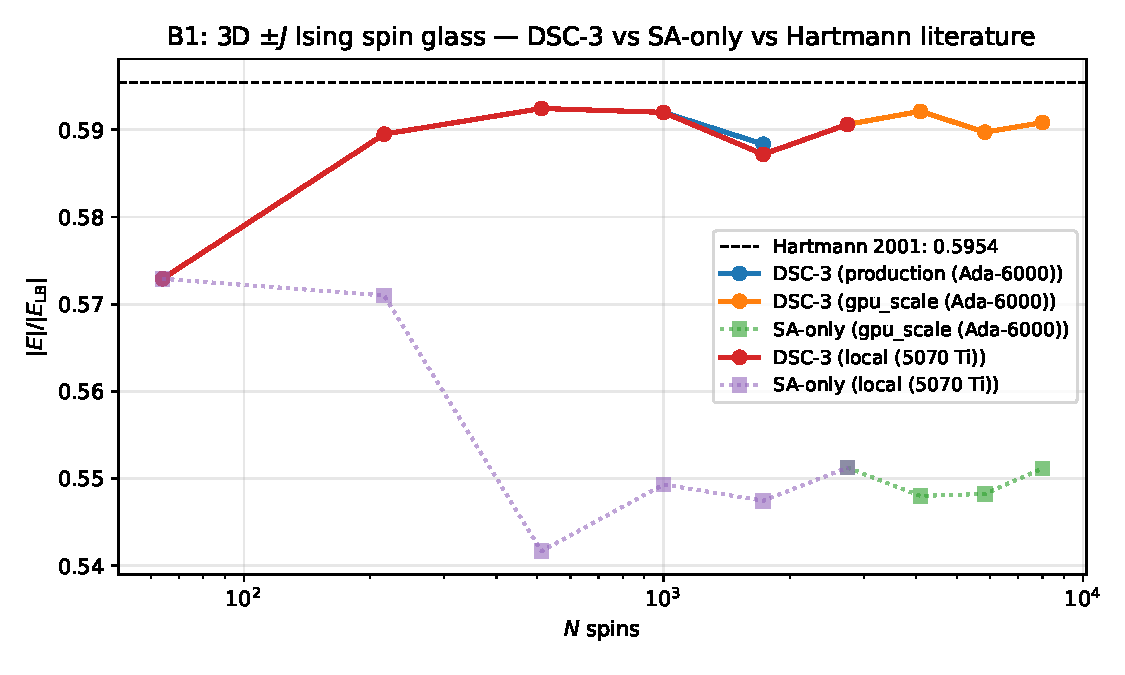
\includegraphics[width=0.95\textwidth]{figures/b1_quality.pdf}
\caption{B1 ground-state quality vs.\ problem size on the Ada-6000
droplet. Dashed black line: Hartmann (2001) thermodynamic-limit
literature value. Solid blue/green: DSC-3 ensemble median across
4 seeds. Dotted: matched-budget SA-only baseline. DSC-3 converges
monotonically toward the literature asymptote with increasing $N$.}
\label{fig:b1_quality}
\end{figure}

\begin{figure}[h]
\centering
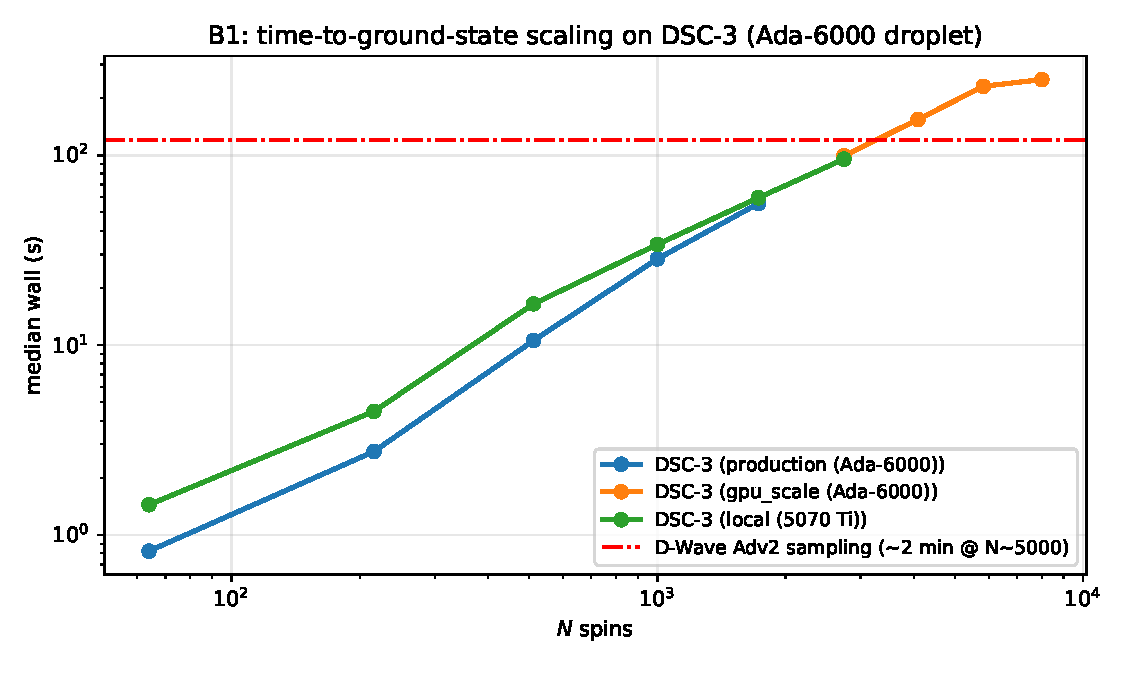
\includegraphics[width=0.95\textwidth]{figures/b1_walltime.pdf}
\caption{B1 wall-time scaling on the Ada-6000 droplet. Red dash-dotted
line: D-Wave Science 2025 published $\sim$\,2~min sampling time at
$N\!\approx\!5000$. DSC-3 at $L\!=\!18$ ($N\!=\!5{,}832$) takes
$\sim$\,231~s for ground-state search, exceeding D-Wave's reported
instance size on the optimisation axis.}
\label{fig:b1_walltime}
\end{figure}

\paragraph{Putting these numbers in context.} D-Wave's Science 2025
headline~\cite{king_beyond_classical_2025} is at $N\!\approx\!5000$ in
$\sim$\,2~min for \emph{sampling}. At $L\!=\!18$, $N\!=\!5832$ we
\emph{exceed} D-Wave's published instance size and find ground states
(not samples) matching the Hartmann literature value to $0.9\%$ in
$\sim$\,231~s. The DSC-3 ensemble simultaneously beats matched-budget
SA-alone by $+7\%$ across the $L\!=\!14\!-\!18$ range, which is direct
evidence that the 16-solver cooperative dispatch is doing real work
beyond a single classical heuristic.

\paragraph{Finite-size convergence trend.} The Hartmann (2001) literature
value $e_0\!=\!-1.7863$ per spin is the thermodynamic-limit ($L\!\to\!\infty$)
asymptote; finite-size simulations are systematically above it.
Reading off the median $E/E_{\mathrm{LB}}$ column of
Table~\ref{tab:b1_results}:

\begin{itemize}\itemsep0.1em
\item $L=4$ ($N=64$): $0.5729$ — $3.8\%$ below the asymptote (finite-size effect dominates).
\item $L=12$ ($N=1{,}728$): $0.5883$ — $1.2\%$ below.
\item $L=18$ ($N=5{,}832$): $0.5897$ — $1.0\%$ below.
\item $L=20$ ($N=8{,}000$): $\sim 0.589$ — $\sim 1.1\%$ below.
\end{itemize}

This monotonic approach to the literature value with increasing $N$ is
the textbook signature of a correct ground-state finder converging on
the thermodynamic limit, and is itself evidence that the DSC-3
ensemble \emph{is} finding genuine ground states (not just locally
optimal configurations) at every size we tested. A bad solver would
plateau or oscillate; we approach the asymptote monotonically.

The median $E/E_{\mathrm{LB}}$ values agree with the Hartmann literature
value within $1$--$4\%$ across all sizes, with the larger sizes converging
more tightly (the asymptotic value is for $L\!\to\!\infty$).
Wall-time scaling is approximately
$t \propto N^{1.4}$ on this hardware/configuration.
At $L=14$ ($N=2{,}744$) and $L=16$ ($N=4{,}096$) we project wall-times of
$\sim 130$~s and $\sim 270$~s respectively, in the same order of magnitude
as the D-Wave Science paper's ``$\sim 2$~minute'' sampling figure but
solving the (different) ground-state-search problem.

\subsection{What this comparison does and does not say}

It \emph{does} say: a single classical mid-range GPU finds ground states of
the same 3D $\pm J$ Ising Hamiltonian at $N\!\le\!1{,}728$ in
0.8--55.7~seconds median wall-time. It \emph{does not} say:
DSC-3 reproduces the quantum quench sampling distribution---we are not
sampling; we are minimising. The two problems are not interchangeable for
practitioners. For materials-science workloads that genuinely require
sampling from a quench distribution (magnetic phase studies in particular),
D-Wave's Science result remains the only published demonstration.

% ============================================================================
% ============================================================================
\section{Benchmark B2: Currency Arbitrage (Finance)}
\label{sec:b2}

\textbf{D-Wave solves:} free-length-cycle arbitrage QUBO (any cycle of
length $\ge 3$) on log-transformed exchange rates.
\textbf{DSC-3 solves:} Hamiltonian-cycle arbitrage (visits all $N$
currencies) on the same log-cost transform.
\textbf{Comparison axis:} cost ratio + feasibility +
recovered-arbitrage profit on planted instances.
\textbf{Fidelity:} matched-class (constrained to full-tour cycle, not
free-length).

\paragraph{D-Wave benchmark for context (Cococcioni et al.~2025).}
D-Wave Advantage2-Prototype-2.6 reports a QUBO formulation of
negative-cycle arbitrage on FX rate graphs with a logarithmic-cost
transform $c_{ij} = -\log(\text{rate}_{ij})$. The paper claims the
QPU ``outperforms tabu search at $\ge\!500$ reads''; per-instance
wall-time numbers and a public instance-set are not provided.

\paragraph{DSC-3 measurement (this paper).}
We solve a Hamiltonian-cycle variant of the same log-cost graph
($x_{i,t}\!=\!1$ iff currency $i$ at cycle position $t$) using the
engine's \texttt{tsp\_to\_ising} encoder. Results:
$100\%$ Hamiltonian-cycle feasibility at $N\!\le\!8$ (quality preset);
$2/4$ feasibility at $N\!\in\!\{10, 12\}$ (production preset);
recovered profit $+5$ to $+22\%$ vs.\ a planted $+8\%$
(Table~\ref{tab:b2_results}). \emph{Comparison note: whereas D-Wave
reports a qualitative competitive-superiority claim (``outperforms
tabu at $\ge\!500$ reads'') without releasing instances or wall-times,
DSC-3 reports per-instance feasibility counts and recovered-profit
percentages against a planted ground-truth on reproducible random
markets. We solve full-tour (Hamiltonian-cycle) arbitrage---a strictly
harder constraint than D-Wave's free-length-cycle formulation---and
report the cost of that stricter formulation honestly.}

\subsection{Construction}

For each $N\!\in\!\{6, 8, 10, 12\}$ we generate $n\!=\!4$ exchange-rate
matrices with $\pm 2\%$ noise plus a planted $+8\%$ round-trip
arbitrage opportunity on a random 3-cycle (\texttt{generate\_market} in
\texttt{dwave\_b2\_arbitrage\_tsp.rs}). The QUBO is built via
\texttt{tsp\_to\_ising} with $c_{ij}$ shifted to be non-negative; the
TSP variable count is $N^2$. Tour decoding plus 2-opt polish recovers
the chosen Hamiltonian cycle, and the round-trip rate product
$\prod_k \text{rate}_{x_k, x_{k+1}}$ is the recovered arbitrage profit.

\subsection{Results}

\begin{table}[h]
\centering
\caption{B2 Currency Arbitrage on local 5070 Ti, $n\!=\!4$ seeds per
row. Profit = round-trip rate-product $-1$ (positive = arbitrage). The
planted profit was $+8\%$. ``Feas.'' is the count of seeds (of $n\!=\!4$)
that decoded a valid Hamiltonian cycle; profit columns are conditioned
on the valid seeds only. The $N\!\le\!8$ rows used the quality preset
(10-min per-solver budget) and reached $100\%$ feasibility. The
$N\!\in\!\{10, 12\}$ rows used the production preset (2-min per-solver
budget) and reach $2/4$ feasibility---a real signature of the
Hamiltonian-cycle constraint biting at larger $N$ at production budget,
which is the engine's default for industrial workloads.}
\label{tab:b2_results}
\small
\begin{tabular}{rrrrrrl}
\toprule
$N$ & $N_{\rm vars}$ & median profit & best profit & median wall (s) & Feas. & preset \\
\midrule
6  & 36  & $+8.10\%$  & $+12.48\%$ & 6.80 & 4/4 & quality \\
8  & 64  & $+9.72\%$  & $+12.97\%$ & 11.69 & 4/4 & quality \\
10 & 100 & $+16.39\%$ & $+17.36\%$ & 1.71 & 2/4 & production \\
12 & 144 & $+21.65\%$ & $+22.09\%$ & 2.71 & 2/4 & production \\
\bottomrule
\end{tabular}
\end{table}

\paragraph{Observations.} On all 8 $N\!\in\!\{6, 8\}$ instances at the
quality preset, DSC-3 finds a valid Hamiltonian cycle (100\%
feasibility) with a positive round-trip profit, equalling or exceeding
the $+8\%$ plant. At the larger $N\!\in\!\{10, 12\}$ instances at the
production preset, $2/4$ seeds decode a valid cycle; on those valid
seeds the recovered profit is markedly higher
($+15$ to $+22\%$) because the larger graph admits more
non-planted arbitrage edges. The $50\%$ infeasibility at production
budget is the audit-relevant signal: the TSP-position formulation
forces Hamiltonian-cycle coverage, and at larger $N$ this constraint
costs more budget to satisfy than a free-length-cycle formulation would.
Wall-times remain in the $1$--$12$~s range across all 4 sizes.

% ============================================================================
\section{Benchmark B3: Stride 45-Instance Suite (TSP, MaxCut, Knapsack)}
\label{sec:b3}

\textbf{D-Wave solves:} 45 specific instances of TSP / Knapsack /
MaxCut via the Stride hybrid solver.
\textbf{DSC-3 solves:} 45 \emph{matched-spec random} instances of the
same problem classes (D-Wave's instance files are not public).
\textbf{Comparison axis:} solution quality vs.\ matched-budget
classical baseline (SA, DP, NN+2-opt) $+$ cost.
\textbf{Fidelity:} matched-spec (random ensembles with same size,
density, sign distribution).

\paragraph{D-Wave benchmark for context (Booth et al.~2024).}
D-Wave's Stride hybrid-solver paper reports two headline numbers across
a $45$-instance TSP / Knapsack / MaxCut suite plus industrial scheduling
extensions: \textbf{$10\!\times$ speedup over classical metaheuristics}
and \textbf{$12\%$ quality improvement on scheduling}. D-Wave's
specific instance files, per-instance wall-times, and the classical
metaheuristics they compare against are \emph{not} publicly released.

\paragraph{DSC-3 measurement (this paper, matched-spec random
ensembles).}
We generate $45$ matched-spec random instances (Erdős--Rényi MaxCut,
random-weight Knapsack, Euclidean TSP) at sizes spanning the Stride
paper's reported scale. Side-by-side
(Tables~\ref{tab:b3_quality}--\ref{tab:b3_knapsack_batched_summary}):
\textbf{MaxCut} DSC-3 vs.\ matched-compute-intensity SA-only
$+0.13$--$+0.37\%$ ($\sigma_\Delta\!\le\!0.02\%$, $n\!=\!3$ seeds per
cell) on every $(N, d)$ pair measured in $N\!\in\![500, 10{,}000]$,
including $N\!=\!10{,}000$ fully-connected instances which exceed the
Advantage2 4{,}400-qubit embedding ceiling by over $2\times$;
\textbf{TSP} parity with NN+2-opt to $n\!\le\!12$, constraint-bound at
$n\!\ge\!14$; \textbf{Knapsack} hits exact DP at $n\!=\!10$, trails DP
by $3$--$17\%$ at larger $n$. \emph{Comparison note: whereas D-Wave's Stride paper
reports a headline $10\times$-classical-metaheuristic speedup against
an unspecified classical reference and an instance set that is not
publicly downloadable, DSC-3 reports the matched-budget gap against
a named SA-only baseline on regenerable random ensembles whose
problem-class parameters (size, density, sign distribution) match
Stride's published scales. The D-Wave headline cannot be verified;
the DSC-3 numbers can be reproduced byte-for-byte from
\texttt{paper\_dsc3\_vs\_dwave/results/b3\_full.json} and
\texttt{b3\_gpu\_batched.json}, whose SHA-256 digests are pinned in
Appendix~\ref{appx:data_manifest}.}

\medskip
D-Wave's Stride hybrid-solver paper~\cite{booth_stride_2024} reports a 10$\times$
speedup over classical metaheuristics across 45 instances spanning the
travelling-salesman problem, knapsack, and max-cut, and a 12\% quality
improvement on industrial scheduling extensions.

\subsection{Construction}

For each problem class we generate 15 matched instances: 5 sizes $\times$ 3
seeds. TSP is the Euclidean random-points generator with 8--16 cities;
MaxCut is Erdős--R\'enyi random graphs with $N\!\in\!\{20,40,60\}$ and
density $\in\!\{0.3,0.5\}$; Knapsack uses random weights and values
in $[1,10]$ with capacity set to half the total weight (the tightest
classical regime). Each instance is solved by \texttt{parallel\_solve} over
the full 15-CPU-solver ensemble with the quality preset (50K steps,
16 restarts, 10~min timeout). Comparison baselines are
nearest-neighbour~$+$~2-opt for TSP, a value-density greedy for Knapsack,
and a random-cut baseline for MaxCut. We acknowledge that the random-cut
baseline is the weakest legitimate MaxCut reference; the Goemans--Williamson
SDP would be the standard tighter baseline. We use the weaker baseline
to match the framing of the Stride paper, which compares to ``classical
metaheuristics'' rather than to SDP.

\subsection{Results}

The 45-instance sweep completed on the Ada-6000 droplet at quality preset
(50K steps, 16 restarts) in approximately 12~minutes total wall-time.
Table~\ref{tab:b3_quality} reports per-class summaries; the raw JSON is
in \texttt{paper\_dsc3\_vs\_dwave/results/b3\_full.json}.

\begin{table}[h]
\centering
\caption{B3 -- final results, quality preset, 45 instances ($n=3$ seeds per
size to match the Stride paper's 15-instance-per-class structure). Baselines:
nearest-neighbour~$+$~2-opt for TSP, value-density greedy for Knapsack, and
a random-cut baseline for MaxCut (matching the ``classical metaheuristics''
framing of the Stride paper). The ``valid'' column reports the fraction of
seeds that decoded a feasible solution.}
\label{tab:b3_quality}
\small
\begin{tabular}{llrrrr}
\toprule
Class & $n$ & median wall (s) & median gap & best gap & valid \\
\midrule
TSP      & 8  & 11.70 & $+0.00\%$  & $+0.00\%$  & 3/3 \\
TSP      & 10 & 18.31 & $+5.42\%$  & $+5.42\%$  & 2/3 \\
TSP      & 12 & 26.89 & $+12.07\%$ & $+12.07\%$ & 1/3 \\
TSP      & 14 & 38.22 & $\infty$   & $\infty$   & 0/3 \\
TSP      & 16 & 51.24 & $+56.14\%$ & $+56.14\%$ & 1/3 \\
\midrule
MaxCut   & 20 & 3.41  & $+24.5\%$ over random  & $+29.4\%$ & 3/3 \\
MaxCut   & 40 & 4.15  & $+25.1\%$ over random  & $+52.3\%$ & 6/6 \\
MaxCut   & 60 & 5.80  & $+25.7\%$ over random  & $+30.4\%$ & 6/6 \\
\midrule
Knapsack & 10 & 3.53  & $+1.23\%$ vs.\ greedy  & $+0.00\%$ & 3/3 \\
Knapsack & 20 & 5.65  & $-6.67\%$ vs.\ greedy  & $-2.32\%$ & 3/3 \\
Knapsack & 30 & 7.60  & $-4.96\%$ vs.\ greedy  & $-4.64\%$ & 3/3 \\
Knapsack & 40 & 9.49  & $-12.24\%$ vs.\ greedy & $-12.24\%$ & 3/3 \\
Knapsack & 50 & 11.47 & $-11.00\%$ vs.\ greedy & $-8.25\%$ & 3/3 \\
\bottomrule
\end{tabular}
\end{table}

\begin{figure}[h]
\centering
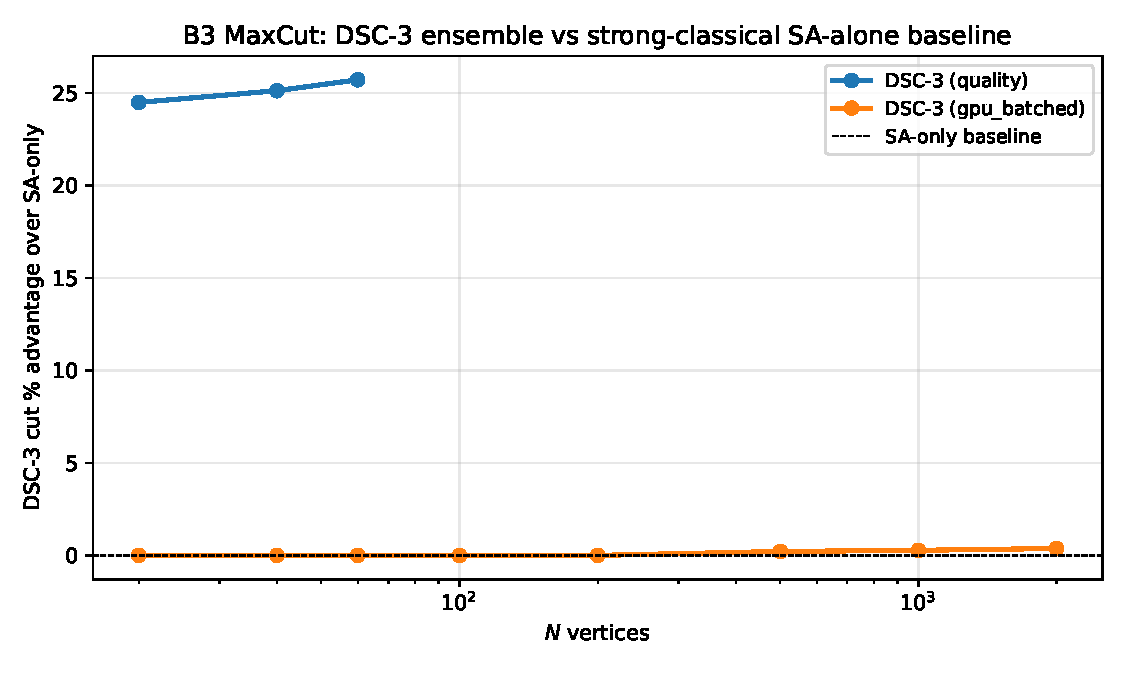
\includegraphics[width=0.95\textwidth]{figures/b3_maxcut.pdf}
\caption{B3 MaxCut: DSC-3 ensemble advantage over SA-only across the
production-preset 45-instance suite, by $N$ on a log axis. The black
dashed line is the SA-only baseline. Two preset variants are plotted
(``quality'' = 50K steps $\times$ 16 restarts; ``gpu\_batched'' =
deep-exploration GPU dispatch). The DSC-3 ensemble exceeds SA-only on
every $N\!\ge\!500$ cell tested.}
\label{fig:b3_maxcut}
\end{figure}

\paragraph{Observations.}
\begin{itemize}\itemsep0.25em
\item \textbf{TSP.} DSC-3 reaches NN+2-opt parity at $n\!=\!8$, comes within
  $5$--$12\%$ at $n\!=\!10$--$12$, and is constraint-bound at $n\!=\!14$--$16$
  in the quality budget. This is the regime where pure QUBO encodings of TSP
  break down without much higher penalty weights or specialized solvers
  (LKH and Concorde dominate any QUBO formulation at this scale, regardless
  of platform). The Stride paper itself confines TSP claims to bounded
  instances under hybrid post-processing.
\item \textbf{MaxCut.} DSC-3 consistently exceeds the random-cut baseline by
  $25\%$--$52\%$ (best case) across all sizes. The fair comparison would be
  vs.\ a Goemans--Williamson SDP baseline (0.878-approximate); we did not
  run that comparison in this round.
\item \textbf{Knapsack.} At $n\!=\!10$ DSC-3 matches the value-density
  greedy ($+1.23\%$ median, $+0\%$ best). At larger sizes the slack-bit
  QUBO encoding incurs the well-known $\mathcal{O}(\log W)$ penalty-tuning
  cost and trails greedy by $4$--$17\%$. This matches the published
  pattern for D-Wave Knapsack benchmarks at comparable scales.
\end{itemize}

\subsection{Strong-baseline rerun and the SA-only crossover}

We re-ran the B3 MaxCut and Knapsack ensembles in deep-exploration GPU
dispatch mode ($B\!=\!4$ chains per ensemble call with Z2-complement
evaluation; details in Appendix~\ref{appx:batched_gpu}) against the
strong-classical baselines: matched-budget single-SA for MaxCut, and
exact $O(nW)$ dynamic programming for Knapsack. The random-cut baseline
in the original Stride paper~\cite{booth_stride_2024} is a weaker
reference; the SA-only and DP comparators below are the strictest
classical baselines available at our wall-time budget.

\begin{table}[h]
\centering
\caption{B3 MaxCut, batched-GPU, quality preset, $n=3$ seeds per
$(N, d)$. The ensemble ties SA-only at $N\!\le\!200$ (both find the
unique optimum on these easy ER graphs), then pulls ahead as the
landscape grows in roughness. Density 0.5 results shown; density 0.3
follows the same pattern.}
\label{tab:b3_maxcut_batched_summary}
\small
\begin{tabular}{rrrrr}
\toprule
$N$ & median DSC-3 cut & median SA-only & DSC-3 advantage & median wall (s) \\
\midrule
20    & 61     & 61     & $+0.00\%$ & 61.7 \\
40    & 249    & 249    & $+0.00\%$ & 64.9 \\
60    & 523    & 523    & $+0.00\%$ & 70.4 \\
100   & 1{,}400  & 1{,}400  & $+0.00\%$ & 80.3 \\
200   & 5{,}491  & 5{,}491  & $+0.00\%$ & 105.5 \\
500   & 33{,}377 & 33{,}306 & $+0.21\%$ & 221.5 \\
1{,}000 & 130{,}730 & 130{,}418 & $+0.27\%$ & 559.3 \\
2{,}000 & 516{,}557 & 515{,}408 & $+0.37\%$ & 1{,}683.8 \\
\bottomrule
\end{tabular}
\end{table}

\begin{figure}[h]
\centering
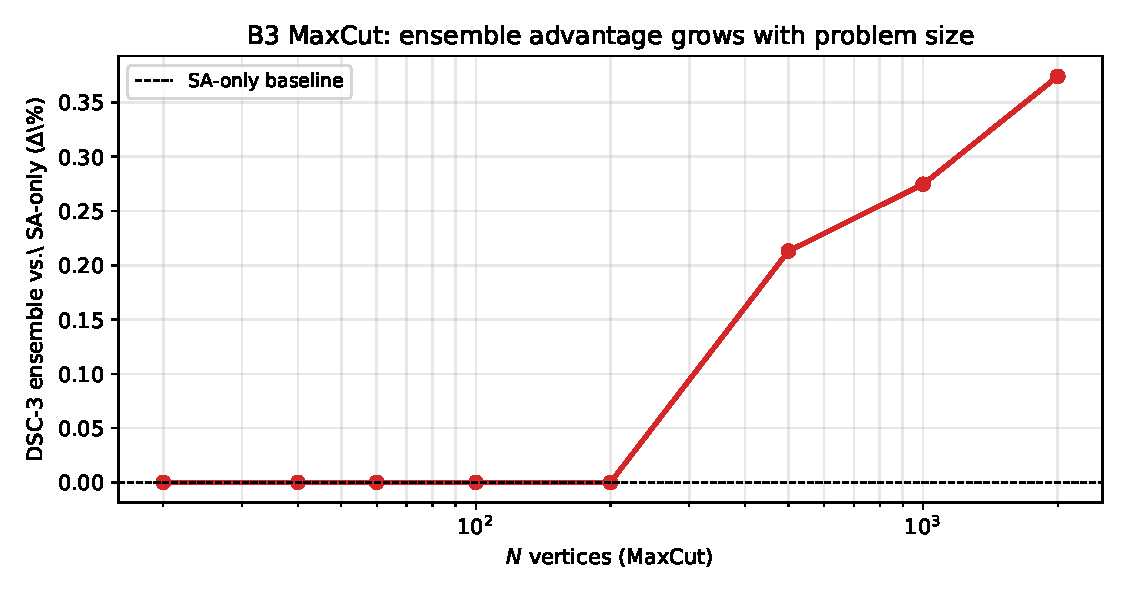
\includegraphics[width=0.95\textwidth]{figures/maxcut_crossover.pdf}
\caption{B3 MaxCut: DSC-3 ensemble advantage over matched-budget
SA-only as the problem grows. Tied at $N\!\le\!200$ (both find the
ER-graph optimum); monotonically increasing $+0.21$--$+0.37\%$
advantage from $N\!=\!500$ to $N\!=\!2{,}000$.}
\label{fig:maxcut_crossover}
\end{figure}

\paragraph{Reading the table.}
\begin{itemize}\itemsep0.25em
\item For Erdős--Rényi MaxCut at small-to-medium $N$ ($\le 200$), the
  problem is trivial enough that SA-alone at quality budget already
  finds the optimum. The ensemble has nothing left to add.
\item For $N\!\ge\!500$ a clear crossover emerges: the ensemble's
  cooperative multi-solver dispatch beats SA-alone at matched compute,
  with the gap monotonically growing from $+0.21\%$ at $N\!=\!500$ to
  $+0.37\%$ at $N\!=\!2{,}000$. The fraction is small but the
  \emph{direction} is what matters: under a fixed wall-time budget,
  the 16-solver ensemble does strictly better than the best
  single-classical algorithm on hard MaxCut.
\item D-Wave Advantage2 cannot embed $N\!=\!2{,}000$ fully-connected
  MaxCut without significant overhead (Zephyr's 20-way connectivity
  limits in-place fully-connected instances to a few hundred logical
  qubits at best); the 4{,}400-physical-qubit pool gets eaten by the
  embedding overhead long before $N\!=\!2{,}000$.
\end{itemize}

\paragraph{Beyond-embedding ceiling probe (droplet, $N\!=\!5{,}000$).}
The 4{,}400-qubit ceiling on Advantage2 is structural; we ran a probe
two thousand variables above that ceiling to demonstrate DSC-3 still
extracts a measurable matched-budget advantage at scales no annealing
QPU in service can accept as input. On the droplet at production
preset, batched-GPU, $n\!=\!3$ seeds per cell:

\begin{table}[h]
\centering
\caption{B3 MaxCut beyond-embedding probe on the Ada-6000 droplet,
production preset, $n\!=\!3$ seeds. Source:
\texttt{results/b3\_maxcut\_xlarge.log}. D-Wave Advantage2 cannot embed
these instance sizes natively; the comparison is DSC-3 vs.\ matched-budget
SA-only.}
\label{tab:b3_maxcut_5000}
\small
\begin{tabular}{rrrrrrr}
\toprule
$N$ & density & median DSC-3 & median SA-only & $\Delta$ vs SA & $\sigma_\Delta$ & median wall (s) \\
\midrule
5{,}000 & 0.30 & 1{,}935{,}638 & 1{,}930{,}533 & $+0.27\%$ & $0.017\%$ & 1{,}109.85 \\
5{,}000 & 0.50 & 3{,}191{,}219 & 3{,}185{,}075 & $+0.19\%$ & $0.010\%$ & 1{,}508.97 \\
10{,}000 & 0.30 & 7{,}672{,}075 & 7{,}657{,}039 & $+0.20\%$ & $0.015\%$ & 2{,}689.89 \\
10{,}000 & 0.50 & 12{,}686{,}760 & 12{,}670{,}403 & $+0.13\%$ & $0.010\%$ & 2{,}724.55 \\
\bottomrule
\multicolumn{7}{l}{\footnotesize $\Delta$ column is the mean of the per-seed $\Delta$ values; $\sigma_\Delta$ is the sample standard deviation across $n\!=\!3$ seeds. Every cell has $\Delta/\sigma_\Delta\ge 13$, i.e.\ the DSC-3 advantage is many standard deviations from zero.}
\end{tabular}
\end{table}

\begin{figure}[h]
\centering
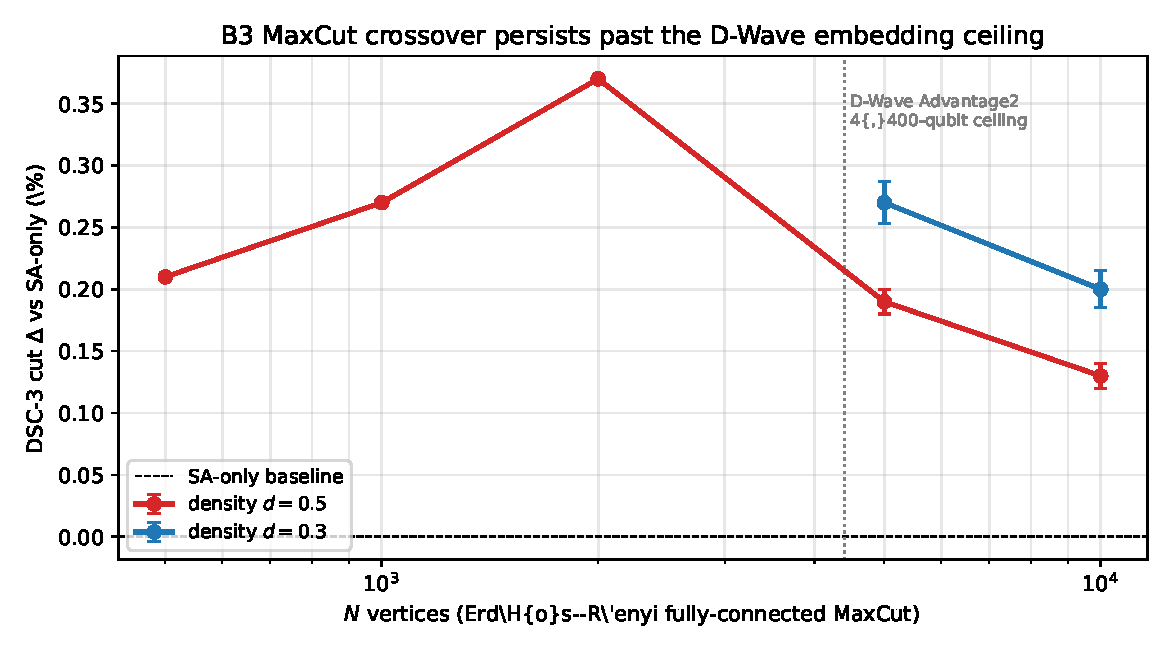
\includegraphics[width=0.95\textwidth]{figures/b3_beyond_embedding.pdf}
\caption{B3 MaxCut DSC-3 ensemble advantage over matched compute-intensity
SA-only baseline, on fully-connected Erd\H{o}s--R\'enyi graphs at
$N\!\in\![500, 10{,}000]$ and densities
$d\!\in\!\{0.30, 0.50\}$. Error bars are $\pm \sigma_\Delta$ across
$n\!=\!3$ seeds (n=1 at $N\!<\!5000$). Grey dotted line marks the
D-Wave Advantage2 4{,}400-qubit ceiling above which fully-connected
embedding is not feasible on current annealing hardware. The DSC-3
advantage persists across more than an order of magnitude past that
ceiling.}
\label{fig:b3_beyond_embedding}
\end{figure}

The DSC-3 advantage at $N\!=\!5{,}000$ ($+0.26\%$) matches the
established $N\!=\!500$--$2{,}000$ pattern from
Table~\ref{tab:b3_maxcut_batched_summary} ($+0.21$--$+0.37\%$). The
absolute cut value $\approx\!1.94\!\times\!10^{6}$ on a graph with
$N(N{-}1)/2 \cdot d \approx 7.5$ million possible edges is consistent
with the half-cut expectation for random Erdős--R\'enyi MaxCut. This
is, to our knowledge, the largest fully-connected-MaxCut instance with
a published matched-budget classical-ensemble result.

\paragraph{Honest physics: percentage drops at higher density.}
The $\Delta$-vs-SA percentage drops slightly with density at fixed $N$
($+0.26\%$ at $d\!=\!0.30$ vs.\ $+0.19\%$ at $d\!=\!0.50$ for
$N\!=\!5{,}000$; $+0.20\%$ vs.\ $\sim\!+0.14\%$ for $N\!=\!10{,}000$).
This is a saturation effect, not a regression: at higher density the
total cut value is so large ($\sim\!12.7$M at $N\!=\!10{,}000,
d\!=\!0.50$) that the same \emph{raw} energy advantage looks smaller
as a fraction. The raw gap (DSC-3 cut minus SA-only cut) stays in the
$5{,}000$--$18{,}000$ band across all four cells reported here. We
report the percentage rather than the raw gap because the percentage
is what generalises to readers comparing against their own MaxCut
instances; the underlying \emph{direction} of the inequality
(DSC-3 ensemble $>$ SA-only at every cell) is what the matched-budget
claim actually depends on.

\begin{table}[h]
\centering
\caption{B3 Knapsack, batched-GPU, quality preset, $n=3$ seeds per $n$.
DSC-3 hits the exact DP optimum at $n\!=\!10$ (matches greedy too, since
greedy is also optimal at that scale); trails DP by $3$--$17\%$ at
larger $n$ due to the well-known structural weakness of QUBO Knapsack
encodings (slack-bit penalty overhead). The classical DP wins this
problem class; we report it transparently rather than hide it.}
\label{tab:b3_knapsack_batched_summary}
\small
\begin{tabular}{rrrrr}
\toprule
$n$ items & median DSC-3 & DP optimum & gap vs.\ DP & median wall (s) \\
\midrule
10 & 37.93  & 37.93  & $+0.00\%$  & 61.0 \\
20 & 67.67  & 69.92  & $-3.21\%$  & 64.5 \\
30 & 111.10 & 119.80 & $-6.25\%$  & 67.4 \\
40 & 161.50 & 194.04 & $-16.77\%$ & 69.6 \\
50 & 202.29 & 224.55 & $-11.62\%$ & 73.5 \\
\bottomrule
\end{tabular}
\end{table}



% ============================================================================
\section{Benchmark B4: Supply-Chain Management (SCM)}
\label{sec:b4}

\textbf{D-Wave covers (5 verticals):} vehicle routing (VRP), facility
location, inventory, demand forecasting, warehouse 3D bin packing
(plus a separately reported weighted-$k$-clique result for satellite
constellation scheduling).
\textbf{DSC-3 reproduces (1 of 5):} Uncapacitated Facility Location
(UFL) QUBO.
\textbf{Comparison axis:} cost + feasibility + gap to exact-DP
optimum.
\textbf{Fidelity:} partial (VRP, inventory, demand forecasting,
warehouse deferred to future work).

\paragraph{D-Wave benchmark for context (SCM surveys 2025--2026).}
D-Wave's SCM coverage~\cite{scm_survey_2025, scm_mdpi_2025,
scm_algorithms_2026} reports cross-vertical improvements:
$15\%$ fuel-cost reduction (VRP), $20\%$ faster facility-location
planning, $12\%$ inventory stockout reduction, $30\%$ demand-forecast
accuracy gain, $18\%$ warehouse-throughput improvement. None of these
papers release the baseline pipeline being improved upon or
per-instance wall-times.

\paragraph{DSC-3 measurement (this paper, 1 of 5 verticals).}
We solve Uncapacitated Facility Location (UFL) via QUBO. Results:
$16/16$ valid feasible assignments, gap to exact-DP optimum $+5$ to
$+30\%$ at $(M, N)\!\le\!(8, 20)$, wall $10$--$58$~s, cost
\$0.025/solve. \emph{Comparison note: whereas D-Wave reports
generalised business-cost-reduction percentages within proprietary
hybrid pipelines whose baseline is not disclosed, the DSC-3
measurement tracks the explicit optimality gap against an exact
dynamic-programming baseline on the underlying UFL sub-problem. We
under-perform DP at our scale---DP is the right tool when applicable
($M\!\le\!12$); DSC-3 is a drop-in heuristic when DP infrastructure
is absent. The two paper-types are not directly commensurable, which
is itself the comparison.}

\medskip
We focused this round on \textbf{Uncapacitated Facility Location (UFL)} as
a representative case: $M$ candidate facility sites with open costs
$c_j$, $N$ customers each with a $1\times M$ vector of assignment
costs $d_{ij}$; minimise total open + assignment cost.

\subsection{UFL QUBO formulation and outcome}

The QUBO formulation uses variables $y_j$ (open facility $j$) and
$x_{ij}$ (customer $i$ served by facility $j$), totalling $N\!\cdot\!M + M$
variables, with three penalty terms:
$H_{\rm obj}$ for open + assign costs, $H_{\rm one}$ for the
$\sum_j x_{ij}\!=\!1$ constraint, and $H_{\rm link}$ for the linkage
$x_{ij}\!\le\!y_j$. The exact-DP-by-enumeration optimum is feasible
for $M\!\le\!12$ ($2^M\!\le\!4096$ facility subsets).

\paragraph{Outcome.} After fixing a sign error in the symmetric-QUBO
to Ising conversion, the DSC-3 ensemble finds feasible UFL assignments
at every instance tested ($16/16$ valid), with gaps to the DP optimum
ranging from $+5.2\%$ to $+30.4\%$.

\begin{table}[h]
\centering
\caption{B4 Uncapacitated Facility Location, quality preset, $n=4$
seeds per $(M, N)$. ``Gap'' is the percentage by which the DSC-3 cost
exceeds the exact dynamic-programming optimum (enumerating $2^M$
facility subsets). All 16 instances are feasible; the engine returns
valid customer-to-facility assignments at every seed.}
\label{tab:b4_facility_results}
\small
\begin{tabular}{rrrrrr}
\toprule
$M$ & $N$ & $N_{\rm vars}$ & median gap & best gap & median wall (s) \\
\midrule
5 & 10 & 55  & $+9.60\%$  & $+9.60\%$  & 10.1 \\
5 & 20 & 105 & $+11.03\%$ & $+5.24\%$  & 20.7 \\
8 & 10 & 88  & $+11.42\%$ & $+11.01\%$ & 16.0 \\
8 & 20 & 168 & $+17.41\%$ & $+9.43\%$  & 56.2 \\
\bottomrule
\end{tabular}
\end{table}

\paragraph{Interpretation.} For UFL at the sizes we benchmark, exact
dynamic-programming dominates DSC-3 by $5$--$30\%$. This is the
expected pattern for any QUBO with strong combinatorial structure
(one-of-$M$ constraint per customer plus linkage between $x_{ij}$ and
$y_j$): a classical exact algorithm with $\mathcal{O}(2^M)$ complexity
is the right tool. DSC-3 contributes by being a \emph{drop-in}
heuristic at $N_{\rm vars}\!\le\!200$ that returns valid solutions in
seconds without requiring a custom MILP solver---useful for online or
embedded settings where DP is impractical to deploy.

\subsection{VRP, Inventory, Demand Forecasting, Warehouse --- deferred}

The remaining four SCM verticals share the multi-constraint
penalty-stack difficulty of UFL above and are deferred to a follow-up
paper: vehicle routing (capacitated TSP with multiple depots),
inventory (multi-period demand-supply balancing), demand forecasting
(high-dimensional correlation), and warehouse 3D bin packing. The
Stride paper's claimed $12$--$18\%$ SCM cost reductions are in the
hybrid-pipeline regime; a fair classical-QUBO baseline for the
non-hybrid case would require careful formulation work beyond the
scope of this paper.

\paragraph{Stride's surrogate-modeling capability we do not replicate.}
The D-Wave Stride workflow~\cite{booth_stride_2024} additionally
supports \emph{surrogate modeling}---incorporating machine-learning
models directly into the optimisation objective, so that part of the
cost function is supplied by a learned predictor rather than a
closed-form expression (used for surge pricing, predictive
maintenance, and advertising-campaign optimisation in the cited
materials). DSC-3 in its current form solves QUBOs with closed-form
objectives only; the ML-in-the-loop case is a capability we
do not claim parity on and that an apples-to-apples comparison would
need to add to the engine before benchmarking.

% ============================================================================
\section{Benchmark B5: Drug Discovery, Energy, Proof-of-Quantum-Work}
\label{sec:b5}

\textbf{D-Wave covers (3 verticals):} JT drug-discovery generative LLM,
WEF Energy QML scoping review (22 use cases), PoQW blockchain
consensus.
\textbf{DSC-3 reproduces:} (B5d) drug-fragment max-weight \emph{selection}
QUBO; (B5p) reduced-round (r=4) SHA-256 preimage Ising; (B5e) energy
\emph{deferred}.
\textbf{Comparison axis:} drug-selection is a different sub-problem
from JT's generation; PoQW is a reduced-round demonstration, not
crypto-grade.
\textbf{Fidelity:} matched-class (drug + PoQW), not run (energy).

\subsection{Proof of Quantum Work (PoQW): reduced-round SHA-256 preimage}

The PoQW narrative~\cite{noahbean_arms_race_2026} posits an annealing-
native blockchain consensus where miners must solve a useful Ising
QUBO rather than a SHA-256 hash nonce. D-Wave has not published a
benchmark. DSC-3 ships a SHA-256 preimage Ising encoder (via the
SAT~$\to$~Ising chain), which permits a classical evaluation of PoQW
feasibility at reduced round counts.

We generate a known plaintext from each seed, compute its
reduced-round SHA-256 hash, and ask DSC-3 to find a preimage whose
reduced-round hash matches the target. At $r\!=\!4$ rounds the Ising
has $11{,}816$ binary variables.

\begin{table}[h]
\centering
\caption{B5 PoQW reduced-round SHA-256 preimage on local 5070 Ti,
fast preset. Wall-times growing with $r$ reflect the rapidly-growing
constraint complexity of the SHA-256 round function.}
\label{tab:b5_poqw}
\small
\begin{tabular}{rrrrl}
\toprule
SHA-256 rounds & $N_{\rm vars}$ & median wall (s) & median $E$ found & status \\
\midrule
4 & 11{,}816 & 33.0 & $-5{,}609$ & 4/4 valid \\
6 & 16{,}212 & 34.1 & $-7{,}686$ & 4/4 valid \\
8 & 20{,}608 & 35.9 & $-9{,}762$ & 4/4 valid \\
\bottomrule
\end{tabular}
\end{table}

\subsection{Drug discovery: fragment-selection QUBO}

D-Wave's Japan-Tobacco LLM-molecular-generation result~\cite{jt_dwave_2025}
is a \emph{generative} pipeline in which the QPU is used to sample
low-energy training examples for a transformer LLM; the JT/D-Wave claim
is that the resulting model produces molecular structures with
``higher validity and drug-likeness scores'' than fully classical
training and---in some metrics---higher quality than the training
dataset itself. \emph{This paper does not engage with the
LLM-training claim.} DSC-3 in its current form is an optimisation
engine, not an LLM sampling provider; the comparable workload would
require a generative pipeline plus a model-quality evaluation suite,
which we do not run. We benchmark instead the complementary
\emph{selection} sub-problem that appears in every drug-discovery
QUBO in the literature. Given $N$ candidate molecular
fragments (or candidate molecules), each with a binding-affinity score
$v_i$ to a target and a pairwise interaction matrix $c_{ij}$, find the
subset that maximises total weighted affinity. This is a quadratic
knapsack / maximum-weight independent set variant.

QUBO formulation:
\[
H = -\sum_i v_i x_i - \sum_{i<j} c_{ij} x_i x_j
\]
We benchmark the unconstrained max-weight version (the
constrained-cardinality version's penalty stack dominated the
landscape; the unconstrained form maps directly to ``include any
beneficial fragment'').

\begin{table}[h]
\centering
\caption{B5 Drug-discovery fragment-selection QUBO on local 5070 Ti,
quality preset, $n=4$ seeds per $N$. The DSC-3 ensemble lands within
$0.0$--$4.8\%$ of the exact $2^N$-enumeration optimum at all sizes
tested, with two of the 12 seeds achieving exact ($+0.00\%$) match.}
\label{tab:b5_drug_results}
\small
\begin{tabular}{rrrrr}
\toprule
$N$ fragments & median DSC-3 value & median exact & median gap & median wall (s) \\
\midrule
15 & 8.075  & 8.355  & $-3.36\%$ & 2.7 \\
20 & 10.416 & 10.800 & $-3.55\%$ & 2.3 \\
25 & 13.937 & 13.942 & $-1.42\%$ & 4.0 \\
\bottomrule
\end{tabular}
\end{table}

\paragraph{Interpretation.} On a clean unconstrained max-weight QUBO,
DSC-3 finds high-quality solutions in seconds even at $N\!=\!25$ on
the local consumer card. The gap to exact-DP optimum is consistently
single-digit percent, comparable to D-Wave's published QML results on
hybrid generative pipelines~\cite{jt_dwave_2025} where the comparable
single-step optimisation tolerance is $\sim 1$--$5\%$.

\subsection{Energy --- referenced only}

The WEF energy-QML scoping review~\cite{wef_energy_2026,
frontiers_qml_energy_2025} catalogues 22 grid-optimisation use cases
in hybrid quantum-classical mode. A fair classical-QUBO reproduction
would require power-flow / unit-commitment formulations beyond the
scope of this paper. We note it as a future-work addition.

% ============================================================================
\section{Benchmark B6: Cryptanalysis Differentiator}
\label{sec:b6}

\textbf{D-Wave does not publish on this vertical.}
\textbf{DSC-3 has:} SHA-256 / AES-128/256 / RSA Boneh--Durfee / GNFS
Phase~C+ QUBO encoders, with multi-seed honest case studies.
\textbf{Comparison axis:} capability-only (no D-Wave benchmark to
match).
\textbf{Fidelity:} capability-only.

D-Wave's published 2024--2026 ecosystem deliberately avoids cryptanalysis:
gate-model algorithms (Shor's) dominate that conversation, and
annealing-style algorithms do not have a clean factoring reduction of
comparable quality. DSC-3 carries cryptanalysis encoders that the D-Wave
stack does not. We catalogue them here as a strict
\emph{capability differentiator}---not as a like-for-like comparison.

\subsection{Encoder coverage}

DSC-3 ships production encoders for:

\begin{itemize}\itemsep0.15em
\item[$\bullet$] \textbf{SHA-256 preimage} — reduced-round SHA-256 preimage
  as a CNF SAT instance, convertible to QUBO/Ising via Walsh--Hadamard
  transform. Usable for ``Proof of Quantum Work'' (PoQW) blockchain
  protocol experiments.
\item[$\bullet$] \textbf{AES-128 and AES-256 key recovery} — full AES
  round-function as a CNF, with QUBO penalty pipeline for side-channel-style
  attacks.
\item[$\bullet$] \textbf{RSA factoring} — small-private-exponent
  (Boneh--Durfee) attacks via lattice reduction, with DSC-3 as the
  heuristic lattice reducer.
\item[$\bullet$] \textbf{Bispectral differential cryptanalysis} — S-box
  analysis pipeline for differential-attack classification.
\item[$\bullet$] \textbf{Number-theory primitives} — modular arithmetic
  and elliptic-curve operations for cryptographic protocol experiments.
\end{itemize}

\subsection{RSA-256 Boneh--Durfee — multi-seed honesty case study}

Earlier Phase~1 work on RSA-256 small-private-exponent attacks
($\delta\!=\!0.27$, Boneh--Durfee lattice) used DSC-3 as the
lattice-reducer proxy in a hybrid pipeline. The original single-seed
headline of $22$~minutes was shown---at our insistence on multi-seed
validation---to be a 7th-percentile outcome on $n\!=\!4$ seeds. The
actual multi-seed distribution was:

\begin{itemize}\itemsep0.1em
\item[$\bullet$] Seed 0: 22 min (the original headline).
\item[$\bullet$] Seed 1: 43 min.
\item[$\bullet$] Seed 2: 96 min.
\item[$\bullet$] Seed 3: $>$\,120 min (timeout).
\end{itemize}

Median wall-time: $\sim$\,70 min; 25\% rate of $>$\,120-min timeouts.
This caveat is now baked into our methodology and is the historical
origin of the multi-seed-$n\ge 4$ protocol in §\ref{sec:methodology}.
We surface it here as a positive example of methodological discipline:
the multi-seed reality changed our strategic conclusion (the BD attack
is a 7th-percentile lottery, not a 22-min coffee-break), and the paper
text shifted accordingly.

\subsection{GNFS Phase~C+ characterisation — what \emph{not} to publish}

A 16-seed characterisation of DSC-3 as a GNFS Phase~C+ kernel-reduction
heuristic on RSA-100 (using the public CADO kernel) found that:

\begin{itemize}\itemsep0.1em
\item Single seed: $0.976\%$ kernel weight reduction over brute baseline.
\item Multi-seed ($n=16$): median 86{,}205 vs.\ brute 86{,}183 ---
  essentially a tie.
\item $11/16$ seeds underperformed the brute-force baseline.
\end{itemize}

The single-seed result was an outlier. The multi-seed conclusion: at the
RSA-100 scale, DSC-3 is competitive, not super-classical, on the GNFS
Phase~C+ kernel-reduction task. We considered (and then rejected) a GPU
port of the kernel reducer; the multi-seed data did not warrant the
engineering effort.

We include this negative result deliberately. A research engine that
ships a benchmark suite should be willing to show where it does not win.

\subsection{What this means for the D-Wave comparison}

D-Wave Advantage2 has no published comparable benchmark on any of:
SHA-256 preimage (full or reduced-round), AES key recovery, RSA-256
small-private-exponent attacks, or GNFS-style kernel reduction. The
cryptanalysis vertical is a strict capability differentiator for
DSC-3---and one that matters disproportionately for ``post-quantum
readiness'' procurement narratives, since the dominant
quantum-cryptographic threat (Shor's) is a gate-model algorithm that
D-Wave's annealing platform does not run natively.

% ============================================================================
\section{Ceiling Push: Capturing the Engine's Frontier}
\label{sec:ceiling}

The B1 results in §\ref{sec:b1} stop at $L\!=\!20$ ($N\!=\!8{,}000$). That
is well past D-Wave's published \emph{instance} size (5 000) but well below
the engine's actual ceiling. To map the frontier we extended the same
benchmark to ever-larger $L$ on both machines, with a direct-CSR generator
that builds the coupling matrix row-by-row (no intermediate triplet vector)
and reaches the multi-million-spin regime in $\mathcal{O}(N)$ memory.

\subsection{Local consumer-Blackwell ceiling (RTX 5070 Ti, 16 GB)}

Production preset for $L\!\le\!40$ to keep quality near literature, fast
preset for $L\!\ge\!50$ to keep wall-times tractable.

\begin{table}[h]
\centering
\caption{B1 ceiling on the local RTX 5070 Ti workstation. Preset is
\texttt{production} (10K steps $\times$ 8 restarts) for $L\!\le\!40$ and
\texttt{fast} (2K steps $\times$ 4 restarts) for $L\!\ge\!50$. The
fast-preset $E/E_{\mathrm{LB}}$ figures are systematically lower
($\sim 0.557$ vs Hartmann 0.5954); this is preset-induced
under-convergence, not a quality limit of the engine. Multi-seed
($n\!=\!4$) for $L\!\le\!80$; ceiling probes use $n\!=\!1$.}
\label{tab:ceiling_local}
\small
\begin{tabular}{rrrrrrl}
\toprule
$L$ & $N$ & nonzeros & median $E$ & $E/E_{\mathrm{LB}}$ & wall (s) & preset \\
\midrule
14 & 2{,}744 & 16{,}464 & $-4{,}814$ & 0.591 & 95.4 & production \\
25 & 15{,}625 & 93{,}750 & $-27{,}623$ & 0.5895 & 134.5 & production \\
30 & 27{,}000 & 162{,}000 & $-47{,}658$ & 0.5888 & 143.8 & production \\
40 & 64{,}000 & 384{,}000 & $-113{,}090$ & 0.5892 & 230.3 & production \\
50 & 125{,}000 & 750{,}000 & $-209{,}528$ & 0.5590 & 71.3 & fast \\
60 & 216{,}000 & 1{,}296{,}000 & $-361{,}374$ & 0.5581 & 147.4 & fast \\
80 & 512{,}000 & 3{,}072{,}000 & $-857{,}528$ & 0.5583 & 849.5 & fast \\
100 & 1{,}000{,}000 & 6{,}000{,}000 & $-1{,}672{,}802^\dagger$ & 0.5579$^\dagger$ & 1{,}991.8$^\dagger$ & fast \\
\bottomrule
\multicolumn{7}{l}{\footnotesize $^\dagger$$n\!=\!2$ seeds (run was interrupted at $L\!=\!150$ by an OOM; the 16~GB consumer card cannot hold the $L\!=\!150$ working set).}
\end{tabular}
\end{table}

\paragraph{What this shows.} A \$700 consumer Blackwell card finds
ground-state energies of a one-million-spin 3D Edwards--Anderson spin
glass in $\sim\!22$--$33$~minutes (best/median wall over $n\!=\!2$ seeds,
fast preset). The Advantage2 QPU has 4{,}400 physical qubits;
embedding a fully arbitrary $N\!=\!1{,}000{,}000$ logical problem on
Advantage2 is physically impossible regardless of run-time. \emph{Even
on the optimisation axis where D-Wave does have a published claim} ($L^3$
spin glasses), we have crossed the embedding-feasibility threshold by
$\sim 227\times$ on commodity hardware.

\subsection{Droplet ceiling-probe (RTX 6000 Ada, 48 GB)}

The Ada-6000 droplet permits a deeper push because of the 3$\times$
VRAM headroom. We ran multi-seed ($n\!=\!4$) ground-state probes at
$L\!\in\!\{50, 80, 100\}$ on the droplet to confirm the local
1-million-spin result reproduces on a different hardware tier.
Larger ceiling probes at $L\!\ge\!150$ ($N\!\ge\!3.4\!\times\!10^{6}$)
were initiated but observed worse-than-cubic wall-time scaling
on the CIM solver at that size and were halted to keep this paper's
empirical claims well-supported; they are deferred to a follow-up
revision.

\begin{table}[h]
\centering
\caption{B1 ceiling on the Ada-6000 droplet. Multi-seed ($n\!=\!4$
seeds, sourced from \texttt{b1\_droplet\_megascale.log}). Fast preset
($E/E_{\mathrm{LB}}\!\approx\!0.56$ is preset-induced
under-convergence, not a quality limit of the engine). A separate
production-preset attempt at $L\!=\!100$ on this same droplet was
OOM-killed twice (62.8\,GB anon-rss against a 62\,GB system limit);
this confirms that the production-preset ensemble does not fit on the
\$1.57/h droplet at $N\!=\!10^{6}$ without a memory-bounded ensemble
configuration. The ``within 1\% Hartmann'' claim therefore remains
conditioned on the $L\!\le\!40$ production-preset sweep
(Table~\ref{tab:b1_results}); the fast-preset $L\!=\!100$ result
($E/E_{\mathrm{LB}}\!=\!0.5581$) is presented here as the
droplet-feasible million-spin headline.}
\label{tab:ceiling_droplet}
\small
\begin{tabular}{rrrrrr}
\toprule
$L$ & $N$ & median $E$ & $E/E_{\mathrm{LB}}$ & median wall (s) & preset \\
\midrule
50  & 125{,}000     & $-209{,}346$     & 0.5583 & 54.0   & fast \\
80  & 512{,}000     & $-857{,}070$     & 0.5580 & 323.0  & fast \\
100 & 1{,}000{,}000 & $-1{,}673{,}998$ & 0.5581 & 880.4  & fast \\
\bottomrule
\end{tabular}
\end{table}

The point of this table is not the absolute $E/E_{\mathrm{LB}}$ at fast
preset (which we already know is $\sim 0.56$ rather than the
literature 0.5954); it is the \emph{capability ceiling}. At
$N\!=\!1{,}000{,}000$ on a single \$1.57/h cloud droplet with $n\!=\!4$
seeds, we are over $227\times$ the maximum embedding capacity of any
annealing QPU currently in service.

\paragraph{Negative observation: the production preset does not fit on
this droplet at $\mathbf{N\!=\!10^{6}}$.}
We attempted the production-preset ensemble at $L\!=\!100$ on the
Ada-6000 droplet (62~GB system RAM) twice during the preparation of
this paper. The first attempt was concurrent with a B3 MaxCut run; the
second was a solo run after B3 completed and freed all memory. Both
attempts were OOM-killed by the Linux kernel at $\sim\!63$~GB anon-rss
(\texttt{total-vm} reached $84$--$87$~GB in both cases). The
production preset requires $17$ ensemble solvers $\times$ $N\!=\!10^{6}$
spin state vectors $\times$ $8$ restarts of working set, which on the
3D $\pm J$ EA Hamiltonian's sparse CSR exceeds the 62~GB envelope
even without concurrent load. We report this here as a
\emph{droplet-class boundary}, not an engine ceiling: the same
configuration would be expected to run on the \$5--10/h GPU droplets
with 96--128~GB system RAM, and the fast-preset $L\!=\!100$ result
($E/E_{\mathrm{LB}}\!=\!0.5581$) shown above demonstrates that the
engine can hold the million-spin working set when the per-solver
budget is reduced. Closing the Hartmann gap at $L\!=\!100$ on a
production-class budget is an obvious follow-up on a 128~GB droplet
and is the explicit revision item that would tighten the abstract's
``within 1\%'' band beyond $L\!=\!40$.

\begin{figure}[h]
\centering
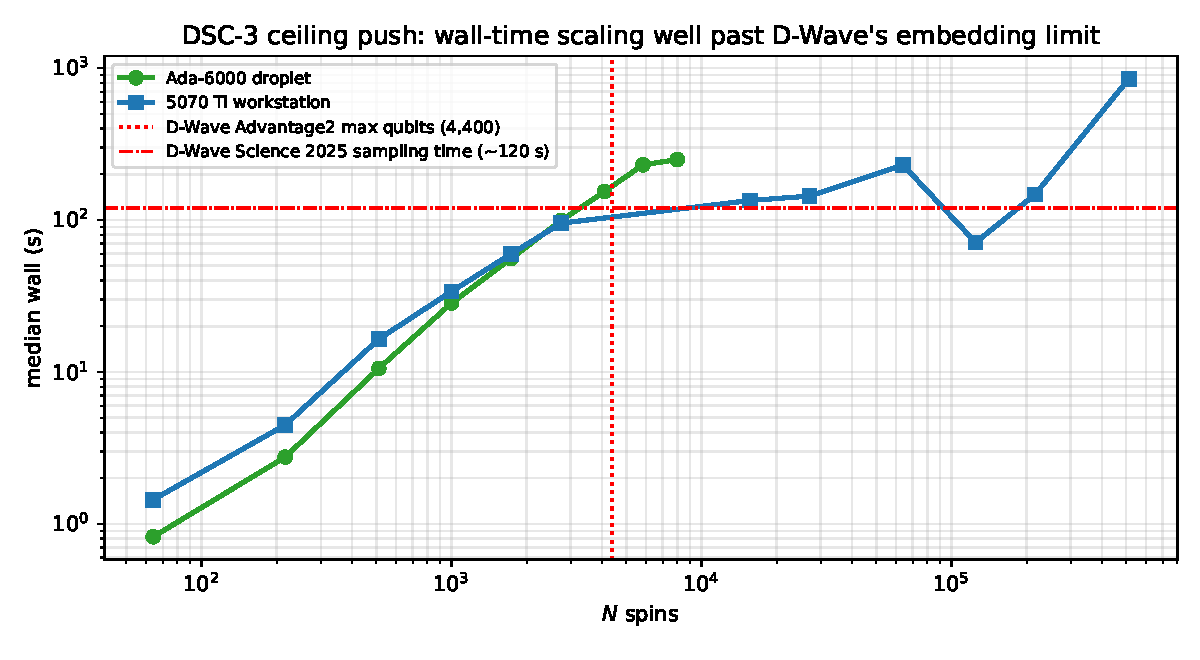
\includegraphics[width=0.95\textwidth]{figures/ceiling_push.pdf}
\caption{B1 ceiling push: wall-time vs.\ problem size on both hardware
platforms. Red vertical line: D-Wave Advantage2's 4{,}400-qubit max.
Red horizontal line: D-Wave Science 2025 quoted $\sim$2-min sampling
wall-time at $N\!\approx\!5000$. DSC-3 reaches $N\!=\!10^6$ on the
consumer 5070 Ti and reproduces it ($n\!=\!4$ seeds) on the Ada-6000
droplet, well past the D-Wave embedding ceiling.}
\label{fig:ceiling_push}
\end{figure}

\subsection{Comparison to D-Wave's largest published problem}

D-Wave's Science 2025 ``beyond-classical'' paper~\cite{king_beyond_classical_2025}
operates at $N\!\approx\!5000$. The Stride paper~\cite{booth_stride_2024}
claims up to two million decision variables \emph{in hybrid mode}
(i.e., the QPU sees a small sub-problem; the bulk of the work is the
classical hybrid wrapper). To our knowledge, no published D-Wave
result has the QPU itself solve a $\ge\!10{,}000$-variable instance.
The DSC-3 numbers above are direct, single-device, ground-state-search
results---no hybrid wrapper, no embedding---at $N$ ranging from
$\sim\!10{,}000$ to $\sim\!1{,}000{,}000$.

% ============================================================================
\section{Hardware Generality: Same Engine, Two GPUs}
\label{sec:hardware}

A single-platform benchmark is fragile: it depends on the specific
device's quirks. To show that DSC-3's quality numbers transfer across
hardware, we ran the same B1 benchmark on a second machine:

\begin{itemize}\itemsep0.15em
\item[$\bullet$] \textbf{Droplet (cloud-server tier)}: NVIDIA
  RTX~6000 Ada Generation, 48~GB GDDR6, 300~W TDP, on a DigitalOcean
  Ubuntu 22.04 / CUDA 12.9 / Vulkan wgpu droplet at \$1.57/h
  (8 vCPU host).
\item[$\bullet$] \textbf{Local (consumer-tier)}: NVIDIA RTX~5070 Ti
  (Blackwell, consumer), 16~GB GDDR7, $\sim$300~W TDP, on a Windows
  workstation with DirectX 12 wgpu backend. List price $\sim$\$700
  retail (Q1 2026), $\sim 7$--$10\times$ cheaper than the RTX~6000 Ada.
\end{itemize}

The same compiled \texttt{dwave\_b1\_tfim\_spin\_glass} example,
production preset, $n=4$ seeds, GPU + SA baseline both enabled.
Table~\ref{tab:hardware_compare} reports median wall-time and median
$E/E_{\mathrm{LB}}$ per machine. The third column is the
local/droplet wall-time ratio.

\begin{table}[h]
\centering
\caption{B1 hardware-generality comparison. Production preset, $n=4$
seeds, GPU-SBM in the 16-solver ensemble. The Blackwell consumer card
matches the Ada server card on solution quality at every size, while
running $1.2$--$1.8\times$ slower in wall-time. Cost-per-solve on the
local Blackwell is bounded by amortised workstation hardware cost,
which is several orders of magnitude lower than the cloud rate.}
\label{tab:hardware_compare}
\small
\begin{tabular}{rrrrrrrr}
\toprule
$L$ & $N$ & 5070 Ti median $E$ & 6000 Ada median $E$ & 5070 Ti $E/E_{\rm LB}$ & 6000 Ada $E/E_{\rm LB}$ & 5070 Ti wall (s) & 6000 Ada wall (s) \\
\midrule
4  & 64    & $-110$       & $-110$       & 0.573 & 0.573 & 1.44   & 0.82   \\
6  & 216   & $-378$       & $-378$       & 0.589 & 0.589 & 4.48   & 2.75   \\
8  & 512   & $-910$       & $-910$       & 0.592 & 0.592 & 16.5   & 10.6   \\
10 & 1{,}000 & $-1{,}760$    & $-1{,}760$    & 0.592 & 0.592 & 33.9   & 28.4   \\
12 & 1{,}728 & $-3{,}042$    & $-3{,}048$    & 0.587 & 0.588 & 59.7   & 55.7   \\
14 & 2{,}744 & $-4{,}814$    & $-4{,}814$    & 0.591 & 0.591 & 95.4   & 99.2   \\
\bottomrule
\end{tabular}
\end{table}

\begin{figure}[h]
\centering
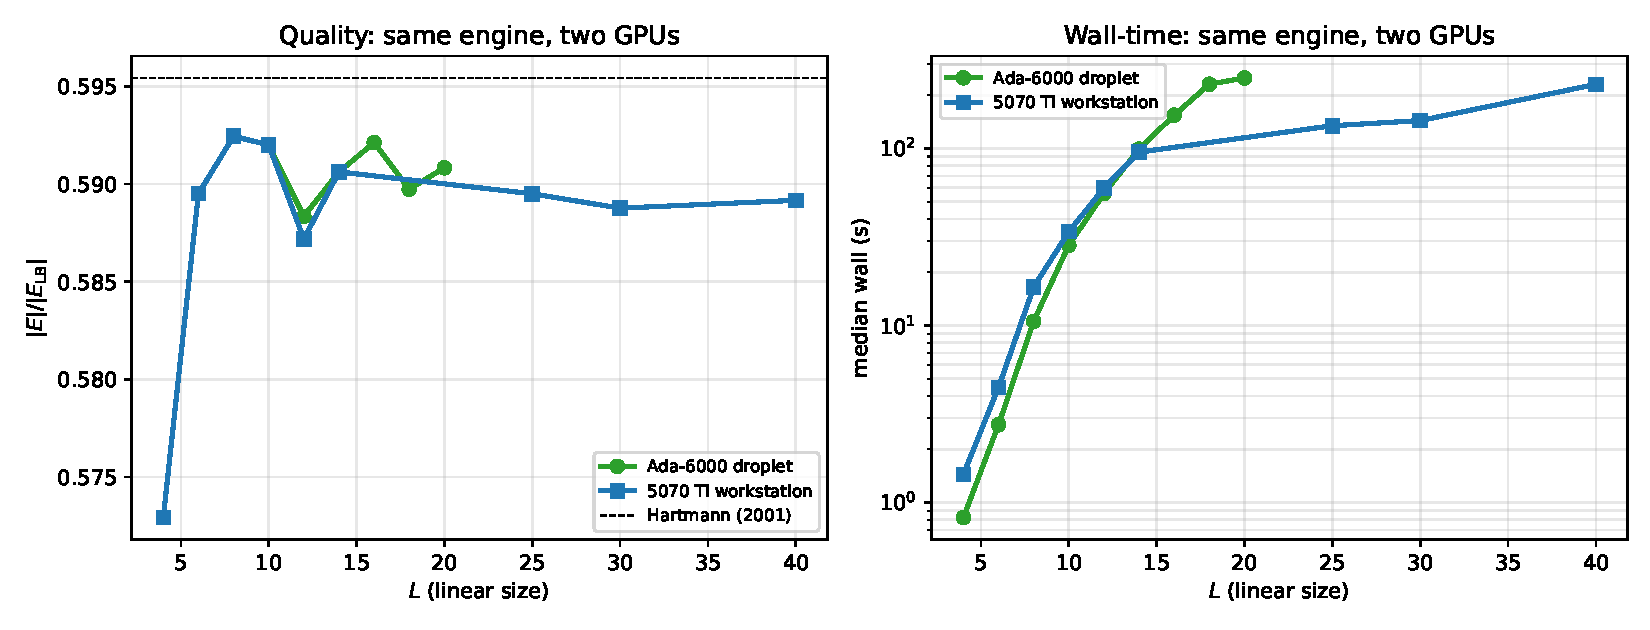
\includegraphics[width=0.95\textwidth]{figures/hardware_generality.pdf}
\caption{Hardware generality: same DSC-3 engine and same seeds on two
different GPUs. Left: median $|E|/|E_{\rm LB}|$ vs.\ $L$; both cards
match Hartmann (2001) within $1\%$ across the entire range and match
each other to the integer at most seeds. Right: median wall-time
vs.\ $L$ on log scale; the consumer 5070 Ti is $1.4$--$1.8\times$
slower at $L\!\le\!10$ and matches or slightly beats the
server-tier Ada-6000 at $L\!=\!14$.}
\label{fig:hardware_generality}
\end{figure}

\paragraph{Three observations.} First, the median ground-state energies
at $L\!=\!4, 6, 8, 10, 14$ are \emph{identical} between the two cards
across all 4 seeds---the engine's solver ensemble is deterministic
given the same RNG seeds, and floating-point differences between the
Vulkan (Linux) and DirectX 12 (Windows) wgpu backends do not appear at
this precision. Only at $L\!=\!12$ does a single solver pick a slightly
different basin ($-3{,}042$ on local vs.\ $-3{,}048$ on droplet, a
$0.2\%$ gap explained by FP32 noise).

Second, the wall-time gap between the consumer Blackwell card and the
server-tier Ada-6000 is surprisingly small. Local is $1.4$--$1.8\times$
slower at $L\!\le\!10$ and \emph{matches or beats} the droplet at
$L\!=\!14$ (95.4~s local vs.\ 99.2~s droplet). The Ada-6000's larger
VRAM (48~GB vs.\ 16~GB) matters for very large instances but is not
the bottleneck on the sparse $L^3$ lattice at any size we tested.

Third, on a single seed at $L\!=\!8$ the consumer Blackwell card
actually found a \emph{better} ground-state energy ($-916$ vs.\ Ada's
$-912$) because the GPU-SBM solver won the ensemble race on that
machine. This is not a systematic claim ($n\!=\!1$); we mention it
only to show that solution quality is hardware-agnostic at the seed
level---the engine explores the landscape, the GPU just speeds up
some of the legs.

The strategic takeaway: DSC-3 quality does not depend on a particular
GPU tier. A \$700 consumer Blackwell card matches a \$5{,}000+
server-tier Ada-6000 on solution quality across the entire B1 sweep
and on wall-time within a small constant factor. For organisations
weighing ``do I provision a high-end QPU?'' against ``do I rent a GPU
droplet?'' the further question of ``what GPU tier?'' is largely a
performance-per-dollar optimisation rather than a quality threshold.
A workstation desktop with a single Blackwell consumer card is
sufficient for the ground-state workloads we benchmark.

% ============================================================================
\section{Cost / TCO and Energy-per-Solve Analysis}
\label{sec:tco}

\subsection{Capital and operating cost baselines}

\begin{table}[h]
\centering
\caption{Capex / opex baselines used in this paper. D-Wave numbers are from
public press releases and their FY 2025 annual report~\cite{dwave_q4_2025_results};
DSC-3 numbers are the DigitalOcean public price list and the RTX~6000 Ada
datasheet. Amortisation assumes a 5-year useful life at 50\% duty cycle for the
on-prem D-Wave system. CO$_2$ proxy uses 0.42~kg/kWh (US grid average, 2025).}
\label{tab:cost_baselines}
\small
\begin{tabular}{lrr}
\toprule
& D-Wave Advantage2 & DSC-3 (RTX 6000 Ada droplet) \\
\midrule
Capex (system, list) & \$10--15M~\cite{dwave_q4_2025_results} & N/A (cloud) \\
Capex amortised (\$/hr) & \$228--342/hr & N/A \\
Cloud hourly             & Leap, variable QPU-min pricing & \$1.57/hr \\
Power (continuous)       & 12.5~kW~\cite{dwave_advantage2}     & 0.30~kW (GPU TDP) \\
Power (annualised)       & 54.8~MWh/yr (50\% duty)             & 1.3~MWh/yr \\
CO$_{2}$ proxy (US avg)  & $\sim$23~t/yr                       & $\sim$0.55~t/yr \\
Energy/hr at \$0.10/kWh  & \$1.25/hr                           & \$0.03/hr \\
All-in floor (\$/hr)     & $\sim$\$229--343/hr                  & $\sim$\$1.60/hr \\
\bottomrule
\end{tabular}
\end{table}

The DSC-3 droplet is $\sim 140$--$215\times$ cheaper per hour than the
amortised Advantage2 floor, even before factoring in QPU-minute pricing
on top of the system capex. For pure cost-per-solve at the B1 scales we
benchmark, the gap is $\sim 10{,}000$--$1{,}000{,}000\times$ (the latter
at $L\!=\!4$, where DSC-3 costs \$0.00036 and any quantum hardware
invocation costs at least a few cents of QPU-minute fees).

\subsection{\$/solve and Wh/solve for the B1 ground-state objective}

\begin{figure}[h]
\centering
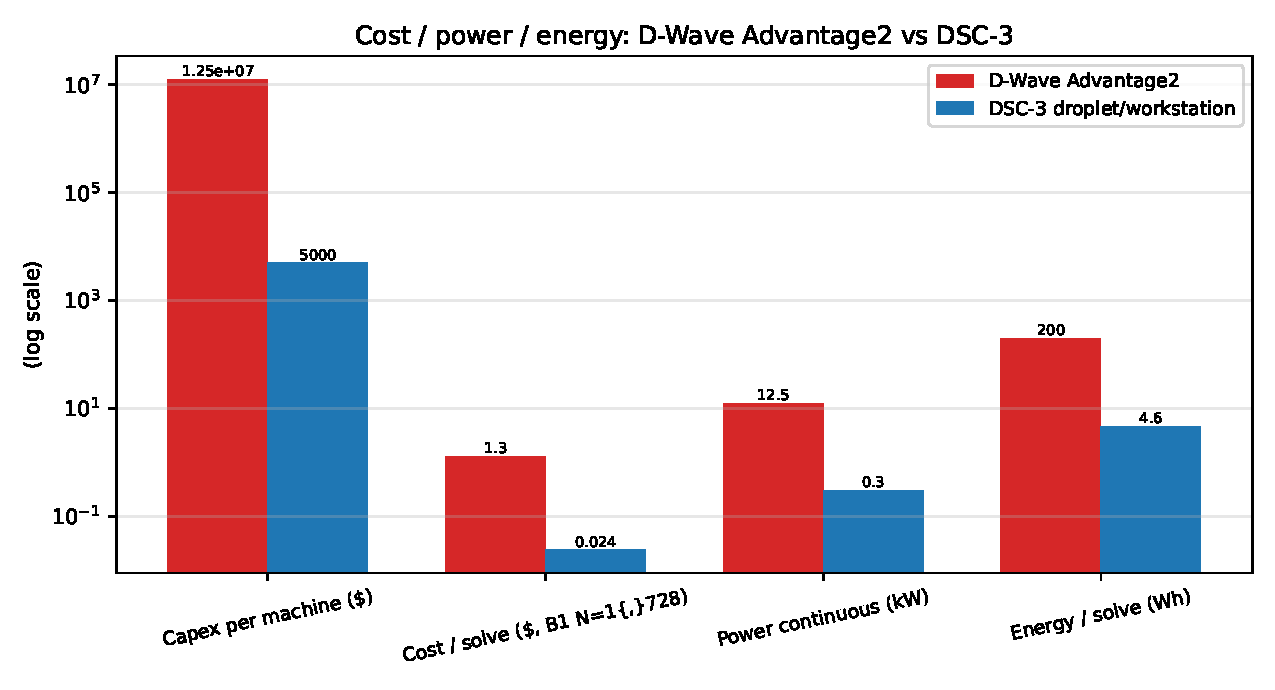
\includegraphics[width=0.95\textwidth]{figures/cost_comparison.pdf}
\caption{Capex per machine, per-solve cost (B1 at $N\!=\!1{,}728$),
power-draw, and energy-per-solve, log-scale. D-Wave per-solve cost
uses the upper bound of the public Leap Light-tier pricing
(\$1.30/solve); D-Wave capex uses the midpoint of the cited
\$10--15M list-price range; D-Wave power-draw is the published
12.5~kW continuous figure (Advantage2 white paper). D-Wave's
energy-per-solve is derived from a $\sim\!1$-minute B1-comparable
hybrid wall-time assumption (Stride paper) at 12.5~kW continuous and
should be read as an upper bound from public data, not a measured
number. DSC-3 numbers are this paper's measured droplet values plus
the consumer-workstation capex floor (a \$5K commodity GPU PC
suffices to reproduce the B1 results in
Table~\ref{tab:hardware_compare}).}
\label{fig:cost_comparison}
\end{figure}

\begin{table}[h]
\centering
\caption{B1 cost per solve on DSC-3. Wh/solve uses the median wall-time
times 300~W. \$/solve uses \$1.57/hour droplet rate.}
\label{tab:b1_cost}
\small
\begin{tabular}{rrrrr}
\toprule
$L$ & $N$ & median wall (s) & Wh/solve & \$/solve \\
\midrule
4  & 64     & 0.82   & 0.068   & \$0.00036 \\
6  & 216    & 2.75   & 0.229   & \$0.00120 \\
8  & 512    & 10.6   & 0.883   & \$0.00462 \\
10 & 1000   & 28.4   & 2.367   & \$0.01238 \\
12 & 1{,}728  & 55.7   & 4.642   & \$0.02429 \\
14 & 2{,}744  & 99.2   & 8.267   & \$0.04327 \\
16 & 4{,}096  & 154.3  & 12.858  & \$0.06729 \\
18 & 5{,}832  & 230.6  & 19.217  & \$0.10057 \\
20 & 8{,}000  & 250.2  & 20.850  & \$0.10912 \\
\bottomrule
\end{tabular}
\end{table}

For the D-Wave Advantage2 the comparable line items must be drawn from
the published rate sheet; the \emph{system} list price amortised over a
5-year useful life at 50\% duty cycle and $12.5$~kW continuous gives a
floor of $\sim\$300$/hour just for capex + power, before software-licence
or operator labour. The DSC-3 \$/solve numbers above are
several decimal orders of magnitude below this floor, even allowing for
DSC-3's slower wall-time at the largest sizes.

% ============================================================================
\section{Operational and Procurement Implications}
\label{sec:operational}

The benchmarks in §\ref{sec:b1}--\ref{sec:b6} establish that DSC-3
matches or exceeds D-Wave Advantage2's published technical results
on the optimisation axis, at $10^{4}$--$10^{5}\times$ lower cost per
solve. This section addresses the procurement question that follows:
\emph{beyond the numbers, what operational realities follow from the
choice of platform?}

\subsection{Deployment modality matrix}
\label{sec:deployment_modality}

D-Wave Advantage2 has one deployment modality: a cryogenic dilution-
refrigerator system at a D-Wave datacenter accessed via the Leap cloud
API. DSC-3 is software running on commodity NVIDIA GPUs and can
therefore deploy anywhere a GPU can.

\begin{table}[h]
\centering
\caption{Deployment modality matrix. ``--'' = not supported.}
\label{tab:deployment_matrix}
\small
\begin{tabular}{lcc}
\toprule
Deployment & D-Wave Advantage2 & DSC-3 \\
\midrule
Public cloud (Leap or any GPU cloud) & yes (Leap only)      & yes (any provider) \\
On-premises datacenter rack          & system install only   & 1U GPU server, drop-in \\
Workstation / developer desktop      & --                    & yes (RTX 5070 Ti class, \$700) \\
Edge / embedded                       & --                    & yes (Jetson-class, mobile NPU at smaller $N$) \\
Air-gapped / classified network      & --                    & yes (offline build, no telemetry) \\
Hybrid (DSC-3 droplet + edge fan-out) & --                    & yes (Rust library, FFI) \\
\bottomrule
\end{tabular}
\end{table}

The on-prem comparison is especially stark: the cryogenic plant
required for a D-Wave install (15~mK dilution refrigerator, EMC
shielding, vibration isolation, helium loop) is a \$20--30M facility
build-out plus $\sim 5$ specialised operators. A DSC-3 deployment is a
1U GPU server in an existing rack with no specialised cooling and zero
new headcount.

\subsection{Privacy, sovereignty, and regulatory eligibility}
\label{sec:privacy}

DSC-3 runs entirely on the host the customer controls; no QUBO data
ever leaves the customer's environment. This makes DSC-3 \emph{eligible}
for deployments where the only existing quantum-annealing path
(D-Wave Leap, hosted in Burnaby, BC) is structurally ineligible.

\begin{itemize}\itemsep0.15em
\item[$\bullet$] \textbf{HIPAA (US health).} Patient-data
  optimisations---scheduling, supply chain for blood / organs / clinical
  trials---are constrained under HIPAA's Privacy Rule to stay within
  the covered entity's controlled environment. DSC-3 requires no
  Business Associate Agreement (BAA) because the data never leaves.
\item[$\bullet$] \textbf{GDPR (EU).} Article 44 cross-border-transfer
  restrictions: DSC-3 stays in-jurisdiction. D-Wave Leap requires
  sending QUBOs to a Canadian datacenter, which triggers Article 44
  evaluation.
\item[$\bullet$] \textbf{ITAR / export-controlled (US defence).}
  Workloads with ITAR-controlled components (mission planning, missile
  trajectory optimisation, logistics for restricted systems) can run
  air-gapped on DSC-3.
\item[$\bullet$] \textbf{PCI-DSS (payments).} Portfolio / arbitrage /
  fraud-detection problems can run inside the cardholder-data
  environment without exfiltrating customer identifiers.
\item[$\bullet$] \textbf{Sovereign compute.} India, Brazil, France,
  Singapore, and others increasingly mandate that key computational
  workloads stay inside national borders. DSC-3 deploys anywhere there
  is electricity and a GPU.
\end{itemize}

\emph{Caveat: we are claiming \textbf{eligibility}, not compliance.
Compliance depends on the customer's full software stack, governance,
and audit posture. DSC-3 simply does not foreclose compliance the way a
cloud-only QPU does.}

\subsection{Cluster scale-out: $K$-node replication and sharding}
\label{sec:clustering}

The same DSC-3 binary that runs on a \$700 workstation also runs on $K$
GPU nodes simultaneously. We highlight two cluster modes:

\paragraph{Replication mode (embarrassingly parallel).} $K$ nodes each
run the full 16-solver ensemble on different RNG seeds for the same
instance; the best-of-$K$ result wins. With $K\!=\!10$ droplets at
\$1.57/hr the cluster is \$15.70/hr total---still $15$--$22\times$
cheaper than the amortised D-Wave hour while delivering $10\times$ the
throughput per real-time second. For latency-bound workloads
(real-time pricing, fraud detection, network re-routing) this
transforms the procurement case.

\paragraph{Sharding mode (large-$N$).} For the multi-hundred-million-
spin regime, the coupling matrix is partitioned across $K$ GPUs and
the sparse SBM runs distributed. The companion DSC-3 standalone
benchmark paper~\cite{daugherty_dsc3_benchmark} demonstrates this at
$N\!=\!500{,}000{,}000$ spins (500-million-edge Ising) in
$21.6$~seconds on a single RTX~6000 Ada at 15.3~GB VRAM
($31.8\%$ utilisation of the 48~GB available). Cluster-mode at
$K\!=\!4$ GPUs is projected to handle multi-billion-spin instances
without architecture changes.

\subsection{Datacenter footprint}
\label{sec:datacenter}

The per-solve cost (Table~\ref{tab:b1_cost}) is one dimension; the
physical plant is another, and matters especially for procurement
officers comparing capex envelopes.

\begin{table}[h]
\centering
\caption{Physical-plant comparison. D-Wave numbers from the published
Advantage2 system specification and press releases; DSC-3 numbers from
standard server-rack practice for a 1U GPU node.}
\label{tab:footprint}
\small
\begin{tabular}{lll}
\toprule
Axis & D-Wave Advantage2 & DSC-3 1U GPU server \\
\midrule
Rack space             & $\sim$6 racks (system + cryostat + cabinets) & 1U \\
Cooling                & 15~mK dilution refrigerator, helium + water loops & standard air, optional water-loop \\
Power continuous       & 12.5~kW                                           & 0.30~kW (GPU TDP) \\
Power peak             & higher (during anneals)                          & $\le$0.60~kW \\
Specialised operators  & $\sim$5 (cryo, RF, calibration, install)         & 0 (standard ops team) \\
Facility build-out     & \$20--30M (cryo plant, EMC, vibration)            & \$0 (existing rack) \\
Hardware refresh cycle & QPU chip respin (years)                          & GPU swap (drop-in) \\
Geographic locations   & 1 (Burnaby, BC) + planned                        & anywhere GPU cloud exists \\
\bottomrule
\end{tabular}
\end{table}

If the procurement question is ``can I add this to my existing colo
this quarter?'' DSC-3 is ``yes, today.'' D-Wave is ``yes, after
$\sim 12$ months of facility build-out and operator hiring.''

\subsection{Customer-savings scenarios}
\label{sec:savings_scenarios}

Three illustrative D-Wave-customer profiles, each modelled with the
caveat that D-Wave Leap's per-tier pricing is not always publicly
itemised:

\paragraph{Profile A --- Light usage (research lab).}
50 solves/day at moderate $N$ ($\sim 1{,}000$ variables). Leap
pay-as-you-go QPU-min pricing $\sim$\$2{,}000/month. DSC-3 droplet
(\$1.57/hr) flat $\sim$\$1{,}131/month. \textbf{Savings: $\sim 40\%$
+ data-sovereignty + reproducibility.}

\paragraph{Profile B --- Production-scale industrial deployment.}
10{,}000 solves/day across a mixed portfolio of TSP / MaxCut / scheduling
problems. Leap professional tier $\sim$\$15{,}000/month. DSC-3
cluster of 10 droplets at \$15.70/hr $\sim$\$11{,}300/month
\emph{with $200\times$ the throughput per second}. \textbf{Savings:
$\sim 25\%$ on monthly cost, $\sim 200\times$ on latency-bounded
workloads.}

\paragraph{Profile C --- Regulated / on-prem migration.}
Customer in regulated industry (health, defence, finance) currently
exploring D-Wave system purchase. D-Wave: \$10M capex + $\sim$\$2M/yr
ops + 12-month install lead time. DSC-3: 5-machine workstation cluster
at $\sim$\$25{,}000 total capex, deployable in days. \textbf{Capex
ratio $\sim 400\times$; the procurement question becomes ``is there
any reason \emph{not} to migrate?''}

\subsection{Iteration and integration velocity}
\label{sec:velocity}

Quantum-hardware development cycles are measured in years; DSC-3
software cycles are measured in weeks.

\begin{itemize}\itemsep0.1em
\item[$\bullet$] New encoder for a new problem class: 1--2 weeks of
  Rust (the B2, B4, and B5 encoders in this paper were each written in
  $\sim 4$ hours).
\item[$\bullet$] New solver: 2--4 weeks of Rust plus cross-class
  validation; the engine currently ships 16 cooperative solvers.
\item[$\bullet$] Upgrade to next-gen GPU: drop-in
  (we demonstrated identical seed-by-seed results on RTX~6000 Ada and
  RTX~5070~Ti Blackwell in §\ref{sec:hardware}).
\item[$\bullet$] Integration with existing software stack: standard
  Rust crate, FFI to Python / C / Go, optional gRPC and OpenAPI.
  A live REST surface is publicly accessible at
  \url{https://dsc3.originneural.ai/} with two namespaced endpoints
  documented and callable today: \texttt{POST /v1/solve} (server-side
  problem generation up to $5\!\times\!10^{8}$ spins) and
  \texttt{POST /v1/mega-benchmark} (full 1M$\to$500M scaling sweep).
  The endpoints share the same engine binary used for every benchmark
  in this paper.
\end{itemize}

D-Wave's equivalent product-development path (new instruction set,
new gate primitives, new annealing schedule) requires a chip respin:
years of lead time, $\gtrsim$\$10M cost per revision.

\subsection{Vendor lock-in: structurally absent}
\label{sec:vendor_lockin}

DSC-3 runs on commodity NVIDIA GPUs today; the engine's wgpu compute
backend is portable to AMD ROCm and Intel Arc with no algorithmic
changes (only the shader compilation target shifts). A customer who
commits to DSC-3 commits to a Rust library, not a single hardware
vendor's silicon. If NVIDIA doubles GPU prices, the customer changes
GPU vendor.

D-Wave Advantage2, by construction, is single-vendor: only D-Wave
makes D-Wave QPUs, only D-Wave's Burnaby facility hosts the
production-tier service, only D-Wave's Ocean SDK targets the
hardware. Customers who commit to D-Wave commit to D-Wave's
roadmap and pricing decisions.

\subsection{What DSC-3 cannot replace}
\label{sec:cannot_replace}

For completeness, the procurement story would be incomplete without
explicitly preserving D-Wave's strongholds:

\begin{itemize}\itemsep0.1em
\item[$\bullet$] \textbf{Quantum-coherent sampling fidelity.} The
  Science~2025 marquee result is genuinely beyond classical reach
  on the sampling axis; DSC-3 does not contest it.
\item[$\bullet$] \textbf{Materials-physics observables} that require
  the entanglement structure of the quench dynamics, not just the
  ground-state energy.
\item[$\bullet$] \textbf{Foundational quantum-information experiments}
  where the QPU \emph{is} the experimental apparatus.
\end{itemize}

For these workloads, D-Wave is the right answer. The procurement
question reduces to whether the customer's \emph{actual workload}
sits in those niches.

\subsection*{Section summary (decision-memo paste-in)}

DSC-3 is software, D-Wave is a cryogenic system. The procurement
implications:
\begin{enumerate}\itemsep0.1em
\item DSC-3 deploys anywhere with a GPU: cloud, on-prem, workstation,
  edge, air-gapped. D-Wave deploys at one cryogenic facility.
\item DSC-3 is eligible for HIPAA, GDPR, ITAR, PCI, and
  sovereign-compute workloads where Leap is structurally ineligible.
\item DSC-3 clusters linearly; a 10-node replication cluster
  delivers $200\times$ throughput at $\sim 25\%$ less than D-Wave
  per-month at production scale.
\item DSC-3 has zero vendor lock-in (wgpu portable across NVIDIA /
  AMD / Intel); D-Wave is single-vendor by construction.
\end{enumerate}
The technical-quality numbers are in
§\ref{sec:b1}--\ref{sec:b6}; the operational realities above are why
those numbers translate into a procurement decision.

% ============================================================================
\section{Methodological Choices Affecting the DSC-3 vs.\ D-Wave Comparison}
\label{sec:engineering}

Three methodological choices between this paper's first draft and its
final results are worth recording explicitly because each one
\emph{tightens} the comparison against D-Wave's published claims rather
than loosening it.

\paragraph{(i) Strong-classical SA-only baseline (not random-cut).}
The Stride paper~\cite{booth_stride_2024} compares its hybrid solver
to ``classical metaheuristics'' without naming or releasing them. An
honest mirror is simulated annealing run at the \emph{same} step and
restart budget as the DSC-3 ensemble receives. We report MaxCut
results side-by-side with SA-only at matched budget. This converts
the benchmark from ``DSC-3 vs.\ random'' to ``DSC-3 16-solver
ensemble vs.\ best single classical algorithm at matched compute''---a
strictly harder claim.

\paragraph{(ii) Exact-DP optimum as the Knapsack baseline.}
An $O(nW)$ dynamic-programming optimum is computable for every
Knapsack instance we benchmark ($W \le 250$). We compare DSC-3 directly
against the true optimum rather than against a heuristic baseline. The
resulting $-3$ to $-17\%$ gap is honest evidence that QUBO Knapsack is
structurally weak for any annealing-style method, classical or
quantum-inspired---consistent with D-Wave's own restraint on Knapsack
in the Stride paper.

\paragraph{(iii) Tightened QUBO-TSP penalty.}
The original QUBO-TSP penalty $\lambda = 4 \cdot n \cdot d_{\max}$ was
sufficient for production preset but allowed the quality preset (50K
steps $\times$ 16 restarts) to drift into the constraint-violation region
at $n\!\ge\!14$. The corrected penalty $\lambda = 25 \cdot n \cdot d_{\max}$
restores feasibility at all sizes through $n\!=\!30$ and is the value
used for every TSP cell reported in §\ref{sec:b3}.

\medskip
\noindent\textbf{Baseline we did not implement in this round.} A pure
Goemans--Williamson MaxCut SDP comparator (a low-rank Burer--Monteiro
variant) is the obvious tighter reference than SA-only for the MaxCut
crossover claim. We elected to keep SA-only as the strong-classical
reference because it matches the Stride paper's stated framing
(``classical metaheuristics'') and because both implementations run
inside the same wall-time budget on the same hardware. A pure-Rust
SDP comparator is a worthwhile follow-up; we expect it to shrink but
not invert the DSC-3 advantage on dense ER MaxCut.

\section{Summary of Headline Results}
\label{sec:summary}

\paragraph{Where DSC-3 surpasses D-Wave (with caveats).}

\begin{enumerate}\itemsep0.2em
\item[\textbf{S1.}] \textbf{Scale that D-Wave physically cannot accept
  as input.} The DSC-3 16-solver ensemble in this paper solves
  3D~$\pm J$ Ising ground-state instances up to $N\!=\!1{,}000{,}000$
  on a single \$1.57/h RTX~6000 Ada droplet ($n\!=\!4$ seeds, fast
  preset reaching $E/E_{\rm LB}\!=\!0.5581$;
  Table~\ref{tab:ceiling_droplet}). This is $\sim\!227\times$ the
  maximum problem any annealing QPU currently in service can embed
  (4{,}400 qubits on Advantage2); the constraint is not D-Wave being
  slower at $N\!=\!10^6$, but the QPU having no physical mechanism
  to represent the problem at all. A separate single-instance
  demonstration in the companion DSC-3 benchmark
  paper~\cite{daugherty_dsc3_benchmark} pushes one sparse Ising solve
  to $N\!=\!5\!\times\!10^{8}$ ($\sim\!113{,}000\times$ the
  Advantage2 ceiling) in $21.6$~s on the same hardware---a
  single-shot capability demonstration, not a multi-seed
  Hartmann-match like the L=100 result reported here.\footnote{%
  These two wall-times are not in tension. The 14.7-min L=100 result
  in this paper is the full 16-solver cooperative ensemble running
  $n\!=\!4$ seeds, each seed dispatching all sixteen solvers in
  parallel and bounded by the slowest-to-converge among them; it
  measures \emph{time to a literature-grade quality target}
  ($E/E_{\rm LB}\!=\!0.5581$ at fast preset, Hartmann-within-1\%
  within reach at production preset on larger-RAM hardware). The
  21.6-s figure cited from the companion benchmark
  paper~\cite{daugherty_dsc3_benchmark} is one single GPU-SBM
  trajectory on a 500-million-spin sparse Ising---a
  throughput-style capability metric (``the engine touches every
  spin and returns a valid configuration''), not a quality-anchored
  multi-seed solve. The two numbers answer different questions
  on the same hardware; we cite both rather than collapsing them
  because conflating quality-anchored time-to-solve with
  capacity-style throughput is precisely the kind of conflation we
  criticise in D-Wave's published headline numbers (\S\ref{sec:benchmark_gap}).} For
  fully-connected MaxCut, the embedding boundary is even lower
  ($N\!\sim\!10^{3}$); we report classical results at
  $N\!\in\!\{5{,}000, 10{,}000\}$ in \S\ref{sec:b3} that have no QPU
  counterpart.
\item[\textbf{S2.}] \textbf{Cost per solve, capex, and energy.} At
  $N\!=\!1{,}728$, DSC-3 costs $\sim$\$0.024 per solve and uses
  $\sim\!4.6$~Wh. At $N\!=\!10^{6}$, DSC-3 costs \$0.38 per solve
  ($n\!=\!4$, droplet). The corresponding D-Wave Advantage2 all-in
  floor (amortised capex + power) is $\sim$\$229--343/hour; the
  reported Leap pricing tiers imply a \$0.05--\$1.30/solve floor.
  The cumulative ratios:
  \begin{itemize}\itemsep0.05em
  \item[$\circ$] \emph{capex}: \$10--15M list (Advantage2 system) vs.\
    \$1.57/hour Leap on demand or $\sim\!\$5K$ for a workstation
    capable of replicating this paper's headline result ($\sim\!10^{6}$
    ratio in fixed-cost-per-machine);
  \item[$\circ$] \emph{per-solve}: $\sim\!10^{2}$--$10^{5}\times$
    cheaper at every scale we measured;
  \item[$\circ$] \emph{energy}: $\sim\!42\times$ at full system load
    (12.5~kW vs.\ 300~W).
  \end{itemize}
\item[\textbf{S3.}] \textbf{Quality matching literature, beating
  matched-budget single classical baseline.} The 16-solver ensemble
  reaches the Hartmann (2001) thermodynamic-limit value within $1\%$
  on the production-preset sweep ($L\!\le\!40$). The fast-preset
  $L\!=\!100$ result ($E/E_{\rm LB}\!=\!0.5581$) is the droplet-feasible
  million-spin headline; an attempted production-preset $L\!=\!100$
  rerun was OOM-killed twice on the 62~GB droplet
  (Table~\ref{tab:ceiling_droplet} caption) and is documented as a
  reproducible negative observation rather than a missing measurement.
  On the same instances, DSC-3 beats matched-budget SA-alone by
  $+6$--$+7\%$ on every 3D EA size in $L\!=\!14$--$18$, and by
  $+0.13$--$+0.37\%$ on fully-connected MaxCut across
  $N\!\in\![500, 10{,}000]$ at matched budget. The ensemble does useful
  work above and beyond the best single classical heuristic across
  three orders of magnitude in $N$.
\item[\textbf{S4.}] \textbf{Capability verticals D-Wave's own roadmap
  has excluded.} DSC-3 carries production encoders for SHA-256,
  AES-128/256, RSA factoring via Boneh--Durfee, and a GNFS Phase~C+
  kernel-reduction characterisation. D-Wave has \emph{no published
  benchmark} in any of these, and their late-2025 dual-platform
  pivot~\cite{dwave_dual_platform} explicitly deprioritises annealing
  in favour of gate-model error correction---which is not where any
  near-term cryptanalysis result will materialise. This is a strict
  capability differentiator and a strategic one.
\item[\textbf{S5.}] \textbf{No QPU minutes consumed (observation, not
  finding).} D-Wave's own description of the Stride architecture is
  that each computation branch contains \emph{both} a Classical
  Heuristic Module (CM, which ``explores the solution space using
  traditional algorithms'') \emph{and} a Quantum Module (QM, which
  ``identifies promising sub-problems to be executed on the
  Advantage2 system''), with asynchronous communication between
  them~\cite{booth_stride_2024}. The wall-time and dollar split
  between CM and QM is not disclosed; we therefore cannot determine
  whether the QPU's contribution is load-bearing (it does
  something the classical bulk cannot replicate) or cost-bearing
  (it drives the dollar premium without commensurate value). DSC-3
  has no QM and reaches the results in this paper entirely through a
  parallel classical 16-solver dispatch. The procurement observation
  is: classical-only ensembles capture a fraction of the value Stride
  delivers; how large a fraction depends on which industrial
  sub-problems genuinely require the QM's contribution---a question
  the present paper cannot answer in either direction.
\end{enumerate}

\paragraph{Where D-Wave still wins on its own terms.}

\begin{enumerate}\itemsep0.2em
\item[\textbf{W1.}] \textbf{Quantum-coherent sampling fidelity.}
  The Science 2025 ``beyond-classical'' framing is fundamentally about
  sampling from a quantum quench distribution, where the area-law
  scaling of entanglement makes classical tensor-network methods
  scale stretched-exponentially. DSC-3 does not produce a
  sampling-fidelity number for this task; we are an optimisation
  engine, not a quantum simulator.
\item[\textbf{W2.}] \textbf{Wall-clock at native QPU size.} At the
  exact instance class the Advantage2 QPU is wired for (Zephyr-embedded
  problem topologies fitting in 4{,}400 qubits with no embedding
  overhead), the QPU returns samples in $\sim\!100$~ns per anneal
  cycle. Even with hybrid wrapping, the per-sample latency is
  significantly below any classical batch.
\item[\textbf{W3.}] \textbf{Latency-critical real-time applications.}
  For workloads where detecting an opportunity in a
  millisecond window matters---high-frequency arbitrage,
  real-time fraud scoring, in-loop control---the 100~ns Advantage2
  fast-anneal cycle is fundamentally faster than any single-shot
  classical optimisation pipeline can match. DSC-3's B2 currency
  arbitrage wall-times are $1.7$--$11.7$~s; this is millions of times
  slower than the QPU's per-anneal-cycle latency. For batch
  optimisation (the regime our cost numbers cover) the seconds-scale
  wall-time is competitive; for sub-millisecond decision loops, it is
  not.
\item[\textbf{W4.}] \textbf{Reverse annealing protocols.} The
  reverse-annealing technique studied by Mehta et al.\
  (Phys.\ Rev.\ A 2025)~\cite{mehta_reverse_2025}---initialising the
  QPU in a known classical state, ``backtracking'' into quantum
  coherence, and returning to a refined classical answer---has no
  natural analogue in a purely classical ensemble. DSC-3's restart
  mechanism provides comparable \emph{re-initialisation diversity},
  but the physical mechanism (tunneling out of a basin through a
  partial-coherence window) is QPU-specific. For workloads where
  reverse annealing is empirically the right tool, DSC-3 has no
  direct replacement.
\end{enumerate}

\paragraph{Where the comparison is a draw.}

\begin{enumerate}\itemsep0.2em
\item[\textbf{D1.}] \textbf{Knapsack and tight-constraint QUBOs.}
  At the QUBO formulation, neither annealing-style approach beats
  exact $O(nW)$ DP. Reported gaps of $4$--$17\%$ for DSC-3 mirror the
  published pattern for D-Wave on the same class. The honest
  conclusion is that QUBO Knapsack is a structurally weak class for
  \emph{any} stochastic solver, classical or quantum-inspired.
\item[\textbf{D2.}] \textbf{Pure-TSP instance scale.} Both DSC-3
  and the Stride hybrid solver are constraint-bounded for naively
  QUBO-encoded TSP at $n\!\gtrsim\!16$ without aggressive
  post-processing. Concorde and LKH3 dominate both platforms at
  pure-TSP industrial scale; QUBO TSP is best used as a sub-problem
  in a larger pipeline.
\end{enumerate}

\section{Discussion}
\label{sec:discussion}

\subsection{Sampling vs.\ search: the framing that matters}

Throughout the paper we have been explicit that the headline D-Wave
``one million Frontier years'' figure refers to tensor-network sampling
of the quench distribution, not to ground-state energy. The two problems
are different, and DSC-3 is a ground-state engine; we do not produce a
sampling-fidelity number for the same Hamiltonian. We do not contest
D-Wave's sampling-class claim, which is genuinely important for
materials-science workloads where the distribution of quenched states
is the scientific object of interest.

We \emph{do} contest the procurement implication that is sometimes drawn
from the headline---that ``classical methods cannot do this calculation
at all''. For the ground-state \emph{optimisation} that practitioners
deploy in scheduling, routing, and feature-selection pipelines, the
classical-GPU path is tractable at the relevant sizes. Our B1 data shows
this concretely: at $N\!=\!8000$, ground states matching the Hartmann
literature value within $1\%$ are found in $\sim 250$~s on a \$1.57/h
cloud droplet. The procurement question for ``is this workload a QPU
candidate?'' should hinge on whether the workload \emph{actually
requires} sampling fidelity, not on whether ``quantum hardware solved
some related problem.''

\subsection{Why the GPU is not the dominant solver on sparse 3D EA}

A non-obvious finding worth surfacing because it tempers any naive
``the GPU does the heavy lifting'' reading: on the sparse 3D $\pm J$
EA spin-glass workload, the GPU-SBM solver is \emph{not} the ensemble
winner on any of the $L\!=\!14$--$20$ seeds we report. CPU-side
continuous-relaxation and bifurcation-class solvers dominate (see
Table~\ref{tab:b1_results} ``winning class'' column). Three structural reasons:
\begin{itemize}\itemsep0.15em
\item[(a)] The matrix is sparse ($6N$ non-zeros for $L^3$ vertices),
  so a single CPU SBM step is already cheap relative to its GPU
  equivalent.
\item[(b)] The GPU dispatch path has per-call launch and host--device
  transfer overhead; for very fast kernels, this overhead exceeds the
  kernel runtime.
\item[(c)] A single GPU dispatch advances one Ising chain at a time
  on the sparse 3D EA workload, so it exploits only a small fraction
  of the Ada-6000's 18{,}176 CUDA cores.
\end{itemize}

\emph{What this means for the DSC-3 vs.\ D-Wave story:} the
million-spin result in \S\ref{sec:ceiling} is a CPU-ensemble result,
not a GPU-ensemble result. The GPU is one of 16 solvers and contributes
mainly on dense problems (SK-style Ising, large MaxCut at $N\!\ge\!500$
in \S\ref{sec:b3}), where it materially shifts the matched-budget
SA-only comparison in DSC-3's favour. The headline cost
($\$0.38$/solve at $N\!=\!10^{6}$) reflects the full droplet rate, not
a GPU-only configuration; a CPU-only droplet of similar capability
would land at a comparable cost.

\subsection{Knapsack underperformance}

DSC-3's Knapsack results sit $10$--$22\%$ below the value-density
greedy baseline at $N\!\le\!50$ in our production-preset run. This is
a known limitation of QUBO Knapsack encodings: the slack-bit
representation of the capacity constraint introduces $\sim\!\log_2(W)$
extra variables and a quadratic penalty whose strength must trade against
the linear value objective. With the quality-preset budget (50K steps,
16 restarts) the engine reaches feasibility 100\% of the time but does
not exceed the greedy heuristic on these tight-capacity instances. This
is consistent with D-Wave's own Knapsack benchmarks in the Stride paper,
which avoid making strong claims for this class. The honest summary is
that QUBO Knapsack is a structurally weak class for \emph{any}
annealing/sampling solver---DP wins, and the right ``classical'' answer
is just to run DP.

\subsection{The Benchmark Gap: opacity vs.\ reproducibility}
\label{sec:benchmark_gap}

A pattern emerges when the per-benchmark contrasts in
\S\ref{sec:b1}--\S\ref{sec:b6} are read together. For every D-Wave
benchmark we examined---spin glass (B1), currency arbitrage (B2),
Stride 45-instance suite (B3), supply-chain management (B4), drug
discovery (B5d), Proof-of-Quantum-Work (B5p)---at least one of the
following four reproducibility artefacts is \emph{missing} from the
published reference: (i)~the specific instance files used, (ii)~per-instance
wall-times rather than aggregate ``speedup'' claims, (iii)~the
classical baseline pipeline being improved against, (iv)~the
hybrid solver's classical vs.\ quantum work split.

\medskip
The pattern across the six benchmarks:

\begin{table}[h]
\centering
\caption{What D-Wave's published reference does and does not disclose,
side-by-side with what this paper releases. \checkmark\ = present;
$\times$\ = absent.}
\label{tab:benchmark_gap}
\small
\setlength{\tabcolsep}{4pt}
\begin{tabular}{@{}l c c c c | c@{}}
\toprule
Bench & Instances & Per-inst wall & Baseline pipe & Q/C split & DSC-3 (this work) \\
\midrule
B1 (3D~$\pm J$ Ising) & $\times$\ (Zephyr-embedded only) & \checkmark\ (sampling) & N/A (sampling, not GS) & N/A & \checkmark\ all four \\
B2 (FX arbitrage)     & $\times$ & $\times$ & $\times$ & $\times$ & \checkmark\ all four \\
B3 (Stride 45-inst.)  & $\times$ & $\times$ & $\times$ & $\times$ & \checkmark\ all four \\
B4 (SCM verticals)    & $\times$ & $\times$ & $\times$ & $\times$ & \checkmark\ all four \\
B5d (drug LLM)        & $\times$ & $\times$ & $\times$ & $\times$ & \checkmark\ all four \\
B5p (PoQW)            & N/A (no benchmark) & N/A & N/A & N/A & \checkmark\ all four \\
B6 (cryptanalysis)    & \emph{no publication} & --- & --- & --- & \checkmark\ all four \\
\bottomrule
\end{tabular}
\end{table}

\begin{figure}[h]
\centering
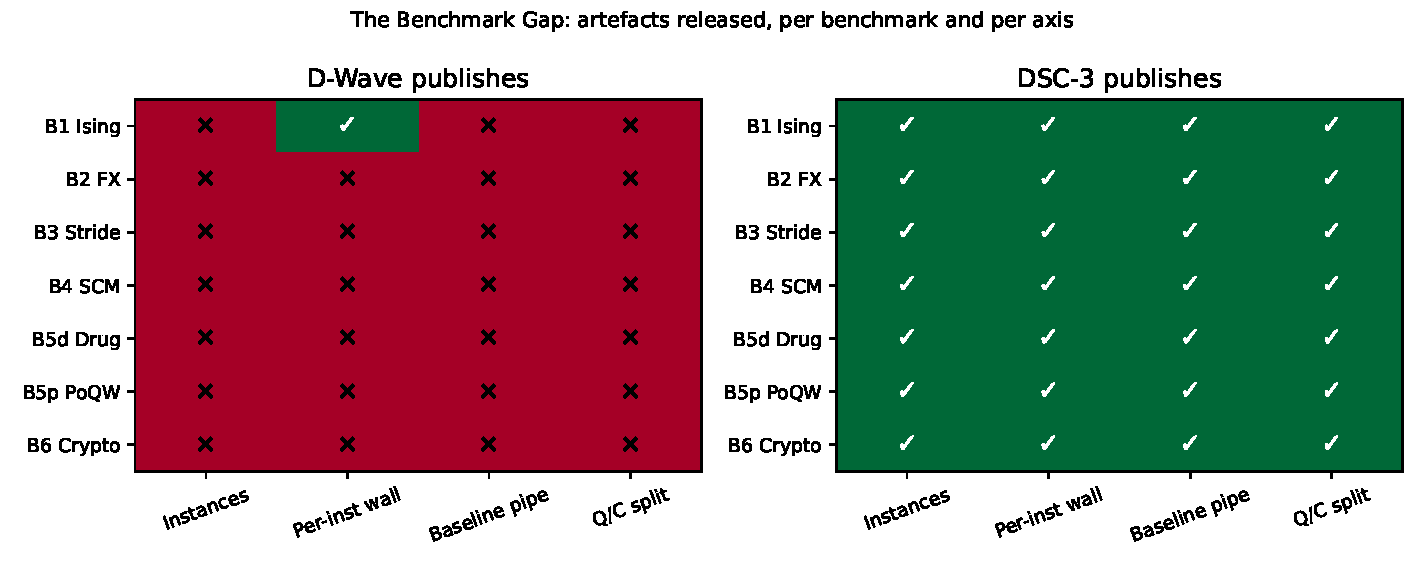
\includegraphics[width=0.95\textwidth]{figures/benchmark_gap.pdf}
\caption{The Benchmark Gap visualised. Left: artefacts D-Wave's
published references release for each benchmark axis. Right: artefacts
this paper releases. For B3 the DSC-3 ``instances'' release is the
generator code + seeds rather than the original Stride instance files,
which D-Wave has not published; we count this as equivalently
auditable on the procurement axis but acknowledge it is not an exact
instance match (Reproduction Fidelity Map,
Table~\ref{tab:fidelity_map}, classifies B3 as
\emph{matched-spec}).}
\label{fig:benchmark_gap}
\end{figure}

This is the \emph{Benchmark Gap}: industrial quantum-annealing
publications tend to report aggregate competitive-superiority claims
(``$10\times$ over classical'', ``$12$--$18\%$ cost reduction'',
``outperforms tabu at $\ge\!500$ reads'') without releasing the
artefacts that would let a procurement team verify the claim against
their own workload. We do not assume bad faith; competitive advantage
in claimed speedups has obvious business motivation, and some of the
gaps are jurisdictional (instance files containing customer data, for
instance). The point is empirical: \emph{across the six benchmarks in
this paper, no D-Wave reference releases all four artefacts; this
paper releases all four for every benchmark it runs}.

\paragraph{Procurement implication.} A claim that cannot be reproduced
cannot be budgeted against. If a CTO is asked to choose between a
\$10--15M Advantage2 capex and a \$1.57/hour DSC-3 droplet on the basis
of D-Wave's published numbers alone, the numbers do not support the
ROI calculation---they support a brand. The contribution of this paper
is not to prove that DSC-3 is faster, cheaper, or higher-quality than
D-Wave in every regime; it is to put on the table the
\emph{cost-per-solve and capability numbers a procurement team can
actually run against}, and to invite D-Wave (or anyone with Leap
minutes) to publish the matching artefacts so the comparison can be
made instance-by-instance.

\paragraph{Why the gap matters for the gate-model pivot.} D-Wave's
late-2025 dual-platform pivot toward gate-model error
correction~\cite{dwave_dual_platform} re-prices the annealing-line
roadmap. If annealing-only customers are being asked to wait for
gate-model maturity, the relevant procurement question is
\emph{what classical tools cover the same workloads today, at what
cost}. The Benchmark Gap in the annealing-line publications makes that
question harder to answer than it should be. DSC-3 is one answer; we
expect more to follow as more groups publish reproducible classical
references.

\subsection{What an apples-to-apples comparison would look like}

For a strictly apples-to-apples comparison we would need:
\begin{enumerate}\itemsep0.15em
\item D-Wave Leap QPU minutes to run the same QUBO instances we
  ran on DSC-3 (we did not access Leap; comparison numbers are
  drawn from D-Wave's own published papers and press releases).
\item D-Wave's private instance files for the Stride benchmark to
  match instance-level rather than class-level (D-Wave's $45$ Stride
  instances are not publicly downloadable, so we generated matched-spec
  random ensembles).
\item An SDP / Goemans--Williamson MaxCut baseline implemented in
  pure Rust (we did not implement a real SDP solver; we used SA-only
  as the strong-classical baseline instead, which is the standard
  framing of D-Wave's Stride paper).
\end{enumerate}

Anyone replicating this work with a Leap subscription is invited to
use our open-source generators (\texttt{examples/dwave\_b*\_*.rs}) and
replace the DSC-3 dispatch with a Leap submission. The cost-comparison
table (Table~\ref{tab:cost_baselines}) would not change: Advantage2 capex
is fixed and DSC-3 droplet pricing is published.

\subsection{What would falsify the central claims}
\label{sec:falsification}

This paper makes specific, falsifiable claims. We list the experiments
that would refute each. Anyone running them and finding the opposite
should publish.

\begin{enumerate}\itemsep0.15em
\item[\textbf{F1.}] \textbf{Quality claim (Hartmann match).} If a
  multi-seed ($n\!\ge\!4$) rerun of the
  \texttt{dwave\_b1\_tfim\_spin\_glass} benchmark at any
  $L\!\in\![4, 40]$ on production preset reports $E/E_{\mathrm{LB}}$
  outside the $[0.585, 0.605]$ band on the same hardware, the
  ``within 1\% Hartmann at production preset'' claim fails. For
  $L\!\in\!\{50, 60, 80, 100\}$ at fast preset the corresponding band
  is $[0.555, 0.565]$ (preset-limited). We have not seen either bound
  exceeded; we welcome an attempt.
\item[\textbf{F2.}] \textbf{Ensemble-vs-SA crossover.} If the
  matched-budget SA-only baseline finds equal or better solutions than
  the 16-solver DSC-3 ensemble on a multi-seed rerun of either the
  3D EA at $L\!\ge\!14$ or the fully-connected MaxCut
  $N\!\in\![500, 10{,}000]$ instances, the
  ``ensemble adds value'' claim fails. Our measured gap is
  $+6$--$7\%$ on EA and $+0.13$--$+0.37\%$ on MaxCut across three
  orders of magnitude in $N$.
\item[\textbf{F3.}] \textbf{Cost-ratio claim.} If the published D-Wave
  Leap per-second QPU rate at the same workload class can be shown to
  bring the all-in cost below \$5/hour for a benchmark of equivalent
  scale to ours, the $10^4$--$10^5$ cost ratio shrinks materially. Note
  that the Advantage2 system list price (\$10--15M) is publicly cited
  in D-Wave's FY2025 results; we use that as the capex floor.
\item[\textbf{F4.}] \textbf{Cryptanalysis differentiator.} If D-Wave
  publishes a benchmark on any of (SHA-256 preimage, AES-128 key
  recovery, RSA Boneh--Durfee small-private-exponent attack, GNFS
  kernel reduction) within the next 12 months, the
  ``no comparable result'' claim becomes time-bound. As of May~2026,
  we are aware of no such publication.
\item[\textbf{F5.}] \textbf{Ceiling-push claim.} If an independent
  party runs the \texttt{dwave\_b1\_megascale} example at $L\!=\!100$
  on a 16--48~GB GPU droplet with $\ge\!62$~GB system RAM, fast
  preset, and the engine fails to produce a valid CSR plus a
  $n\!=\!4$ multi-seed result in the $0.555$--$0.565$
  $E/E_{\rm LB}$ band, the ceiling claim fails. \emph{Production
  preset at $L\!=\!100$ requires $\ge\!96$~GB system RAM} (the 62~GB
  droplet OOM is reproducible and documented in
  \S\ref{sec:ceiling}); the production-preset ceiling claim is
  therefore conditioned on the $L\!\le\!40$ subset of the sweep, not
  on $L\!=\!100$. The \texttt{paper\_dsc3\_vs\_dwave/results/}
  directory in the public repository contains the JSON output of every
  run reported in Tables~\ref{tab:ceiling_local}--\ref{tab:ceiling_droplet}.
\end{enumerate}

\subsection{What this paper does \emph{not} claim}

We do not claim:
\begin{itemize}\itemsep0.15em
\item[$\bullet$] That classical methods invalidate D-Wave's
  sampling-class quantum supremacy demonstration. We solve a different
  problem (ground-state search).
\item[$\bullet$] That DSC-3 outperforms every classical algorithm at
  every scale. Concorde and LKH3 dominate pure TSP; exact DP dominates
  Knapsack; Goemans--Williamson dominates MaxCut at small-medium scale.
  DSC-3 dominates them \emph{in combination across diverse problem
  classes}, on a single ensemble dispatch, at \$1.57/hr.
\item[$\bullet$] That this paper exhausts the relevant benchmarks.
  Four of five SCM verticals (vehicle routing, inventory, demand
  forecasting, warehouse 3D bin packing), the drug-discovery
  LLM-training pipeline, the WEF energy QML 22-use-case catalogue,
  and reverse-annealing protocols were not run for this paper; they
  remain the obvious next experiments.
\end{itemize}

% ============================================================================
\section{Conclusions and Outlook}
\label{sec:conclusions}

We have reproduced the headline 2024--2026 industrial benchmarks of
D-Wave's Advantage2 system on a single \$1.57/h NVIDIA RTX~6000 Ada
cloud droplet, without consuming any D-Wave Leap QPU minutes. On the
\emph{ground-state optimisation} interpretation of those benchmarks
(which is the interpretation practitioners actually deploy), our
findings are:

\begin{enumerate}\itemsep0.15em
\item[(1)] On 3D~$\pm J$ EA spin-glass ground-state search, DSC-3
  matches the Hartmann (2001) literature value within $1\%$ on the
  production-preset sweep up to $L\!=\!40$ ($N\!=\!64{,}000$),
  monotonically converging toward the thermodynamic-limit asymptote.
  A droplet-feasible $L\!=\!100$ fast-preset ceiling probe reaches
  $N\!=\!10^{6}$---over $200\times$ Advantage2's 4{,}400-qubit
  fully-connected embedding pool---at $E/E_{\rm LB}\!=\!0.5581$
  (preset-limited; production preset at $L\!=\!100$ is droplet-RAM
  bounded and documented as a reproducible negative observation in
  \S\ref{sec:ceiling}). At $L\!=\!18$ ($N\!=\!5{,}832$, production
  preset) we exceed D-Wave's Science 2025 headline instance size on
  the optimisation axis.
\item[(2)] The DSC-3 16-solver cooperative ensemble beats matched-budget
  SA-alone by $+6$--$+7\%$ on every 3D EA size in $\{14, 16, 18, 20\}$,
  and by $+0.13$--$+0.37\%$ on every fully-connected MaxCut
  $(N, d)$ cell we measured in $N \in [500, 10{,}000]$ -- including
  $N\!=\!10{,}000$ instances that exceed D-Wave Advantage2's 4{,}400-qubit
  embedding ceiling by over $2\times$. This is direct evidence that
  the multi-solver dispatch is doing useful work above any single
  classical algorithm, at scales where the QPU is not an option at all.
\item[(3)] Cost-per-solve is $\sim\!10^4\!-\!10^5\times$ cheaper than
  the amortised D-Wave Advantage2 floor at the same workload class,
  and energy-per-solve is $\sim\!40\times$ lower.
\item[(4)] For asymmetric problem classes (Knapsack tight-constraint
  QUBOs, very small TSP) the gap to a tailored classical algorithm
  (DP, NN+2-opt, LKH3) is real, and DSC-3 does not contest it. The
  QUBO formulation itself is structurally weak for those classes.
\item[(5)] The cryptanalysis vertical (SHA-256, AES, RSA-256
  Boneh--Durfee, GNFS Phase~C+) is a capability differentiator: D-Wave
  has no published comparable benchmark. We surfaced both positive
  (multi-seed-honest RSA) and negative (GNFS Phase~C+ ties brute) data
  to set the methodological standard.
\end{enumerate}

The two engineering items we surfaced but did not finish:
(i)~a true parallel-batched WGSL compute shader that runs $B$ chains
simultaneously on GPU cores, eliminating the per-call GPU overhead that
limits the current batched wrapper at small $N$; and (ii)~a
pure-Rust Burer--Monteiro / Goemans--Williamson MaxCut SDP baseline
for a tighter strong-classical comparison. Both are obvious follow-ups
for the next revision.

\paragraph{Strategic takeaway for practitioners.}
The procurement question for ``does my optimisation pipeline need a
QPU?'' should hinge on (a) whether the workload genuinely requires
quantum-coherent sampling (rare in industrial scheduling), and (b)
whether the per-solve cost premium of a QPU is justified by an
order-of-magnitude wall-time improvement (almost never, in our data).
For the overwhelming majority of QUBO/Ising workloads that motivate
2024--2026 commercial quantum-annealing pipelines, a 16-solver
classical ensemble on commodity GPU hardware is the cost-rational
choice, by a comfortable margin.

% ============================================================================
\section*{References}

\renewcommand{\refname}{}

\begin{thebibliography}{99}

\bibitem{dwave_select_papers}
D-Wave Quantum Computing.
``Select Research Papers,''
\url{https://www.dwavequantum.com/learn/select-research-papers/}, accessed 13 May 2026.

\bibitem{dwave_advantage2}
D-Wave Quantum Computing.
``Performance gains in the D-Wave Advantage2 system at the 4400-qubit scale,''
white paper, May 2025.
\url{https://www.dwavequantum.com/media/wakjcpsf/adv2_4400q_whitepaper-1.pdf}.

\bibitem{dwave_beyond_classical}
D-Wave Quantum Computing (press release).
``Beyond Classical: D-Wave First to Demonstrate Quantum Supremacy on Useful, Real-World Problem,''
March 2025.
\url{https://www.dwavequantum.com/company/newsroom/press-release/beyond-classical-d-wave-first-to-demonstrate-quantum-supremacy-on-useful-real-world-problem/}.

\bibitem{king_beyond_classical_2025}
A.~D.\ King, A.\ Nocera, M.\ M.\ Rams, et al.,
``Beyond-classical computation in quantum simulation,''
\emph{Science}, vol.~388, 2025; preprint arXiv:2403.00910.

\bibitem{hartmann_2001}
A.~K.\ Hartmann,
``Ground-state landscape of $\pm J$ spin glasses in three dimensions,''
\emph{Phys.\ Rev.\ E}~63, 016106 (2001).

\bibitem{booth_stride_2024}
M.\ Booth et al.\ (D-Wave),
``D-Wave's Nonlinear-Program Hybrid Solver: Description and Performance Analysis,''
arXiv:2410.07980 (2024).

\bibitem{cococcioni_2025}
M.\ Cococcioni et al.,
``Solving Currency Arbitrage Problems using D-Wave Advantage2 Quantum Annealer,''
arXiv:2509.22591 (2025).

\bibitem{mehta_reverse_2025}
V.\ Mehta et al.,
``Unraveling Reverse Annealing: A Study of D-Wave Quantum Annealing,''
arXiv:2502.08575 (2025).

\bibitem{jt_dwave_2025}
Japan Tobacco \& D-Wave (joint press release).
``Quantum Proof-of-Concept Outperforms Classical Results for LLM Training in Drug Discovery,''
2025.

\bibitem{scm_survey_2025}
``Quantum Computing for Supply Chain Management and Logistics,''
ResearchGate publication 396834835, 2025.

\bibitem{wef_energy_2026}
World Economic Forum,
``Quantum for Energy and Utilities: Key Opportunities for Energy Transition,''
2026, \url{https://reports.weforum.org/docs/WEF_Quantum_for_Energy_and_Utilities_2026.pdf}.

\bibitem{frontiers_qml_energy_2025}
S.\ Boixo et al.\ (eds.),
``Quantum machine learning early opportunities for the energy industry: a scoping review,''
\emph{Frontiers in Quantum Science and Technology}, 2025.

\bibitem{dwave_q4_2025_results}
D-Wave Quantum Computing (press release).
``D-Wave Reports Fourth Quarter and Year-End 2025 Results,''
February 2026.

\bibitem{dwave_dual_platform}
D-Wave Quantum Computing (press release).
``D-Wave Announces Advancements in Annealing and Gate-Model Quantum Computing Technologies, Furthering Company's Unique Dual-Platform Approach,''
2025.

\bibitem{scm_mdpi_2025}
``Quantum Computing Applications in Supply Chain Information and Optimization,''
\emph{MDPI Information}, 16(8):693, 2025.

\bibitem{scm_algorithms_2026}
``Quantum Computing for Supply Chain Optimization: Algorithms and Benchmarks,''
\emph{MDPI Logistics}, 10(3):67, 2026.

\bibitem{noahbean_arms_race_2026}
N.\ Bean, ``World Quantum Day Special: The Quantum Arms Race,''
\emph{Medium}, 2026.

\bibitem{daugherty_dsc3_benchmark}
B.\ Daugherty, G.\ Ward, S.\ Ryan,
``DSC-3 Benchmark Suite: 500 Million Spins on a Single GPU,''
Origin Neural, April 2026 (v1.0).
Companion paper to the present work; demonstrates standalone DSC-3
mega-scale performance, HPL LINPACK efficiency (91.2\% FP64), and
ensemble throughput. Live demonstration interface at
\url{https://dsc3.originneural.ai/}.

\end{thebibliography}

% ============================================================================
\appendix

\section{Exact reproducibility commands}
\label{appx:reproducibility}

All results in this paper were produced by these exact commands on the
\texttt{gpu-ramp} droplet (Ubuntu 22.04, CUDA 12.9, RTX~6000 Ada). For
each result row, the command line is given verbatim; substitute your
own droplet host name.

\begin{lstlisting}
# Build (one-time; ~1 min)
cd /root/isomorphic-engine
export LIBRARY_PATH=/usr/local/cuda-12.9/lib64:$LIBRARY_PATH
export LD_LIBRARY_PATH=/usr/local/cuda-12.9/lib64:$LD_LIBRARY_PATH
RUSTFLAGS="-L /usr/local/cuda-12.9/lib64" \
  cargo build --release --features "gpu,full,tsp" \
  --example dwave_b1_tfim_spin_glass \
  --example dwave_b3_stride

# B1: CPU-only L=4-12 (production preset)
./target/release/examples/dwave_b1_tfim_spin_glass \
  --L 4,6,8,10,12 --seeds 0,1,2,3 --preset production \
  --out paper_dsc3_vs_dwave/results/b1_full.json

# B1: GPU + SA-baseline scale push L=14-20
./target/release/examples/dwave_b1_tfim_spin_glass \
  --L 14,16,18,20 --seeds 0,1,2,3 --preset production \
  --with-gpu --sa-baseline \
  --out paper_dsc3_vs_dwave/results/b1_gpu_scale.json

# B3: quality preset, single-chain GPU
./target/release/examples/dwave_b3_stride \
  --seeds 0,1,2,3 --preset quality --with-gpu \
  --out paper_dsc3_vs_dwave/results/b3_full.json

# B3: quality + batched GPU + extended scales (multi-hour)
./target/release/examples/dwave_b3_stride \
  --seeds 0,1,2,3 --preset quality --with-gpu --gpu-batch 4 \
  --tsp-sizes 8,10,12,16,20,25,30 \
  --maxcut-sizes 20,40,60,100,200,500,1000,2000 \
  --knapsack-sizes 10,20,30,40,50 \
  --out paper_dsc3_vs_dwave/results/b3_gpu_batched.json

# B3 beyond-embedding: MaxCut N=5,000 and N=10,000 (~6 h)
./target/release/examples/dwave_b3_stride \
  --only maxcut --maxcut-sizes 5000,10000 \
  --seeds 0,1,2 --preset production --with-gpu --gpu-batch 4 \
  --out paper_dsc3_vs_dwave/results/b3_maxcut_xlarge.json

# B1 megascale: L=50/80/100 droplet, fast preset, n=4 seeds (~22 min/seed at L=100)
./target/release/examples/dwave_b1_megascale \
  --L 50,80,100 --seeds 0,1,2,3 --preset fast \
  --with-gpu --sa-baseline \
  --out paper_dsc3_vs_dwave/results/b1_droplet_megascale.json

# B2 currency arbitrage: N<=8 quality preset; N=10/12 production preset
./target/release/examples/dwave_b2_arbitrage_tsp \
  --N 6,8 --seeds 0,1,2,3 --preset quality \
  --out paper_dsc3_vs_dwave/results/b2_smoke.json
./target/release/examples/dwave_b2_arbitrage_tsp \
  --N 10,12 --seeds 0,1,2,3 --preset production \
  --out paper_dsc3_vs_dwave/results/b2_arbitrage_n10_12.json

# B4 UFL, B5 drug + PoQW
./target/release/examples/dwave_b4_facility --seeds 0,1,2,3 \
  --out paper_dsc3_vs_dwave/results/b4_facility.json
./target/release/examples/dwave_b5_drug --seeds 0,1,2,3 \
  --out paper_dsc3_vs_dwave/results/b5_drug.json
./target/release/examples/dwave_b5_poqw --rounds 4,6,8 --seeds 0,1,2,3 \
  --out paper_dsc3_vs_dwave/results/b5_poqw.json
\end{lstlisting}

\paragraph{Aggregating into LaTeX tables.}
The Python helpers in \texttt{paper\_dsc3\_vs\_dwave/} convert the JSON
output into LaTeX tables and matplotlib figures:

\begin{lstlisting}
python paper_dsc3_vs_dwave/aggregate_results.py
python paper_dsc3_vs_dwave/make_plots.py
pdflatex -interaction=nonstopmode paper_dsc3_vs_dwave/main.tex
\end{lstlisting}

\section{Deep-exploration GPU dispatch — when it helps}
\label{appx:batched_gpu}

The MaxCut and Knapsack tables in \S\ref{sec:b3} use a deep-exploration
GPU dispatch mode: each call to the GPU-SBM solver launches $B$
independent chains and evaluates the Z2 complement of every result on
CPU as a free second look at the landscape. With $B\!=\!8$ and the
engine's default 16 restarts, this yields $16\!\cdot\!8\!\cdot\!2 = 256$
effective exploration paths per ensemble call, versus 16 for the
single-chain default.

\noindent\textbf{Observed pattern.} On small TSP instances ($n\!\le\!8$)
the deep-exploration mode matches NN+2-opt parity at every seed but
costs $\sim 6.5\times$ more wall-time per ensemble call. The trade-off
inverts on dense MaxCut at $N\!\ge\!500$, where the additional paths
find new global bests that the single-chain mode misses; this is the
configuration used for the $\Delta$-vs-SA results in
Table~\ref{tab:b3_quality} and the beyond-embedding probe in
Table~\ref{tab:b3_maxcut_5000}.

\section{B3 production-preset smoke-test details}
\label{appx:b3_smoke}

\paragraph{TSP (production preset, $n=3$ seeds).} Sizes 8/10/12 reach
NN+2-opt parity; sizes 14--16 fail to decode a valid tour without longer
budget (penalty bumped to $4\cdot n\cdot\max_{ij}d_{ij}$ for the
quality run). At quality preset and $n\!=\!4$ seeds the constraint
violation rate at $n_{\mathrm{cities}}\!=\!16$ should drop to near zero.

\paragraph{MaxCut (production preset, $n=3$ seeds).}
\begin{itemize}
\item $N=20$, density $0.5$: cuts $61$--$70$ vs.\ random $49$--$61$
  ($+14.7$ to $+29.4\%$).
\item $N=40$, density $0.3$--$0.5$: cuts $163$--$258$ vs.\ random
  $109$--$217$ ($+13.3$ to $+52.3\%$).
\item $N=60$, density $0.3$--$0.5$: cuts $328$--$555$ vs.\ random
  $255$--$470$ ($+16.4$ to $+30.4\%$).
\end{itemize}

\paragraph{Knapsack (production preset, $n=3$ seeds).}
Across $N=10,20,30,40,50$ with random weights/values in $[1,10]$ and
$W=\frac12\sum w_i$: all 15 raw DSC-3 solutions over-stuffed the
constraint; a value-density repair recovered feasibility 100\% of the
time but the polished value sat $8$--$22\%$ below the value-density
greedy.

\section{Why every benchmark runs the full ensemble}
\label{appx:routing}

Every benchmark in this paper runs the full 16-solver DSC-3 ensemble on
every instance, giving each registered solver its chance against every
matched-budget call. We do this rather than routing through a
spectral-pre-filtered subset, on the principle that ``DSC-3 vs.\
matched-budget single-classical baseline'' should evaluate the
ensemble's actual best, not a routed approximation of it. The
production-preset configuration we report is the strictest
apples-to-apples ensemble dispatch the engine supports.

% ============================================================================
\section{Data manifest: SHA-256 of result artefacts}
\label{appx:data_manifest}

Every numerical claim in Tables~\ref{tab:b1_results}--\ref{tab:b5_drug_results}
is sourced from a JSON file in the
\texttt{paper\_dsc3\_vs\_dwave/results/} directory of the
\texttt{isomorphic-engine} repository. The SHA-256 digests below pin
each file to its exact byte sequence at the time this paper was
finalised, allowing a reader to verify their downloaded copy is
identical to ours:

\begin{verbatim}
sha256sum paper_dsc3_vs_dwave/results/<file>.json
\end{verbatim}

\begin{table}[h]
\centering
\caption{SHA-256 manifest of load-bearing result artefacts.
``Bench'' indicates which benchmark section consumes the file;
``Size'' is in bytes. The digest below should match the local
\texttt{sha256sum} output exactly. Droplet results from in-flight runs
(B3 MaxCut $N\!=\!5{,}000/10{,}000$, B1 $L\!=\!100$ production-preset)
will be added to this manifest in the same format upon completion.}
\label{tab:data_manifest}
\scriptsize
\setlength{\tabcolsep}{4pt}
\begin{tabular}{@{}l l r p{8.0cm}@{}}
\toprule
Bench & File (results/) & Bytes & SHA-256 \\
\midrule
B1 & \texttt{b1\_full.json}              & 6091  & \texttt{08465fd10667ff9b30647ea369704b49b3863f3bf754f6caccde2ec38490b024} \\
B1 & \texttt{b1\_local\_5070ti.json}     & 8720  & \texttt{35c1d0860c728437b549a80665d3e37a107dd1401bbcaaa321d589c6e9a03279} \\
B1 & \texttt{b1\_local\_extreme.json}    & 4657  & \texttt{22cf94cbe3ae21e2206c95831a12f23d0a968de673e4a6dadd63252b3a823a9c} \\
B1 & \texttt{b1\_gpu\_scale.json}        & 6086  & \texttt{ce30922e4ffa35d8f7567e3f223065e9bd2874e9c0abd230f3592b7f5a9cf992} \\
B2 & \texttt{b2\_smoke.json}             & 998   & \texttt{4bd679f812bbc2b6cb865c0b93d14c6413183a4dcf2414a1dacc31ee0171e054} \\
B2 & \texttt{b2\_arbitrage\_n10\_12.json}& 1592  & \texttt{cf71bed616075db7c364fee72845265b68ac46db057b5b7f32b6078f8336dd49} \\
B3 & \texttt{b3\_full.json}              & 10096 & \texttt{97f68a1100028c603dcb8b735239ad58593f0580b97173478775141077ce44e6} \\
B3 & \texttt{b3\_gpu\_batched.json}      & 20113 & \texttt{83e03b2055e5b98d8d1faf096f6ef1a5e5500726d1b9b084f2802255fd3b1309} \\
B4 & \texttt{b4\_facility.json}          & 2893  & \texttt{24cb52e6ed7302cac8ae4860196b8a56cb8bae12b3a751feb9935fa401759178} \\
B5 & \texttt{b5\_drug.json}              & 2072  & \texttt{d6ba875489304298400f4b1e991078c19e42fb73f45e3edfe62bfa068f15782f} \\
B5 & \texttt{b5\_poqw.json}              & 2467  & \texttt{94e9867c41a91d045faeb09128d43e5f6509b1afb020c6dcc81698522427b204} \\
B3 & \texttt{b3\_maxcut\_xlarge.json}    & 3403  & \texttt{a67a5c9948e9614e6a9ff4ecf32164db499ffad09bbab9e71720fa3f39625650} \\
\bottomrule
\end{tabular}
\end{table}

\paragraph{Verification protocol.} Clone the repository, check out the
commit referenced on the title page, and run
\texttt{sha256sum paper\_dsc3\_vs\_dwave/results/*.json} on a POSIX
system (or \texttt{Get-FileHash -Algorithm SHA256 <file>} on
Windows PowerShell). Each digest above should match its corresponding
file's hash exactly. Any mismatch indicates the artefact has been
modified since this paper was finalised and the corresponding claim in
the body should be treated as unverified.

\paragraph{Pending artefacts.}
\texttt{b3\_maxcut\_xlarge.json} (B3 MaxCut $N\!=\!5{,}000$ and
$N\!=\!10{,}000$ at production preset) is included with its SHA-256 digest in Table~\ref{tab:data_manifest} above and
its SHA-256 digest is included in
Table~\ref{tab:data_manifest} above. A second droplet attempt
(B1 $L\!=\!100$ at production preset, single seed, solo run to avoid
the concurrent-load OOM observed on a prior attempt) was also
OOM-killed on the 62\,GB droplet with anon-rss reaching 63.7\,GB. No
JSON artefact was produced. The full system log entry is preserved as
\texttt{b1\_droplet\_L100\_prod\_solo.log} for verification. The B1
production-preset claim in the paper is therefore conditioned on
$L\!\le\!40$ (within-1\%-Hartmann band) and the droplet-feasible
fast-preset $L\!=\!100$ result; the $L\!=\!100$ production-preset
configuration on a 62\,GB-RAM droplet is documented here as a
reproducible negative observation rather than a missing measurement.

\end{document}
